\newpage
\section{Umsetzung}

Das Ziel ist das Erkennen und Labeln von Objekten in einer AR Umgebung, durch Image Based Object Detection.

\subsection{Design des Vorgang der Objekternennung}

Im Folgenden werden die Arbeitsschritte einer Detection beschrieben.

Wenn der Nutzer das Signal gibt, beginnt die Detection. Als Erstes wird ein Foto mit der Kamera der AR Brille aufgenommen. 
Dieses Foto wird dann an Azure Object Detection und Azure Custom Vision geschickt. 
Die Services untersuchen das Foto nach Objekten, geben deren Klasse und Position auf dem Foto an.

Für jedes Objekt soll ein Label erstellt werden, das zeigt wo sich das Objekt in der realen Welt befindet.
Dafür wird in der 3D Szene der AR Umgebung eine virtuelle Repräsentation des Fotos erschaffen. Die Fotorepräsentation muss die richtige Skalierung, Position und Rotation haben, um das räumliche Verhältnis zwischen der realen Foto-Kamera und der Umgebung nachzubilden.

Da die Fotokamera und das Display nahe beieinander liegen und den gleichen Blickwinkel haben, kann die Position des Displays als Repräsentation des Fotos genutzt werden. In der 3D Szene ist das Display mit der Hauptkamera gleichgesetzt. Die Clipping Plane der Kamera hat somit die gleiche Rotation und eine zumindest ähnliche Position und Skalierung wie das Foto. 

Daher werden die Foto-Positionen auf Koordinaten der Clipping Plane abgebildet. Dabei werden verbleibende Positions- und Skalierungsunterschiede ausgeglichen. Für jedes Objekte wird so eine Koordinate auf der Clipping Plane bestimmt. 

Als Nächstes wird ein Raycast, von der Kamera aus, durch die Clipping Plane Koordinate geschickt. Der Raycast schneidet sich mit einem Mesh, das die reale Welt abbildet. Die getroffene Position wird mit einem Schriftzug markiert. Dort befindet sich das Objekt, das auf dem Foto gefunden wurde.

Alle Objekte, die Azure Object Detection und Azure Custom Vision gefunden haben, werden so für den Nutzer in der AR Umgebung markiert.

\subsection{Architektur}

Die Magic Leap One übernimmt alle Berechnungen im 3D Raum und führt Spatial Mapping durch. Da die Analyse von 2D Fotos sehr speicher- und rechenintensiv ist, wird sie an eine REST-API delegiert. Die Magic Leap wird als Interaktionsmöglichkeiten für den Nutzer verwendet, nimmt die RGB-Fotos der Umgebung auf, liefert diese an die REST-API und zeigt die Ergebnisse und Zwischenstände der Objekterkennung mit UI Elementen in der Szene an. Siehe Abbildung \ref{dia:flow}

\begin{figure}[H]
	\centering
	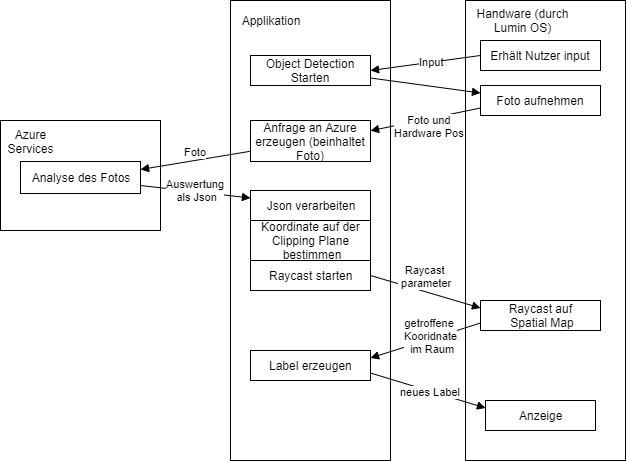
\includegraphics[width=1\textwidth]{images/dia_flow.png}
	\caption[Diagramm der Architektur]{Diagramm der Architektur inklusive Bearbeitungsschritte und Informationsweitergabe.}
	\label{dia:flow}
\end{figure}

% https://developer.magicleap.com/en-us/learn/guides/get-started-developing-in-unity
Das Projekt wurde in Unity umgesetzt und für die Magic Leap AR Brille entwickelt.
Es wurde das Unity Project Template von Magic Leap verwendet. 

Zusätzlich werden einige vorgefertigte Klassen von Magic Leap verwendet. Dazu gehören MLInput, MLCamera, MLRaycast, MLPrivilegeRequestBehavior und MLSpatialMapper. Diese Klassen greifen auf Funktionalitäten des Lumin OS zu.

Die benötigten Funktionalitäten für die Integration der Object Detection mit der REST-API wurde in mehreren Script Klassen umgesetzt. Der Großteil der Scripts verhält sich wie Singletons. Sie existieren nur einmalig in der Szene.

Das Klassendiagramm auf Abbildung \ref{dia:classdiagramm} zeigt die Scripts und ihre Relationen zueinander.

\begin{figure}[H]
	\centering
	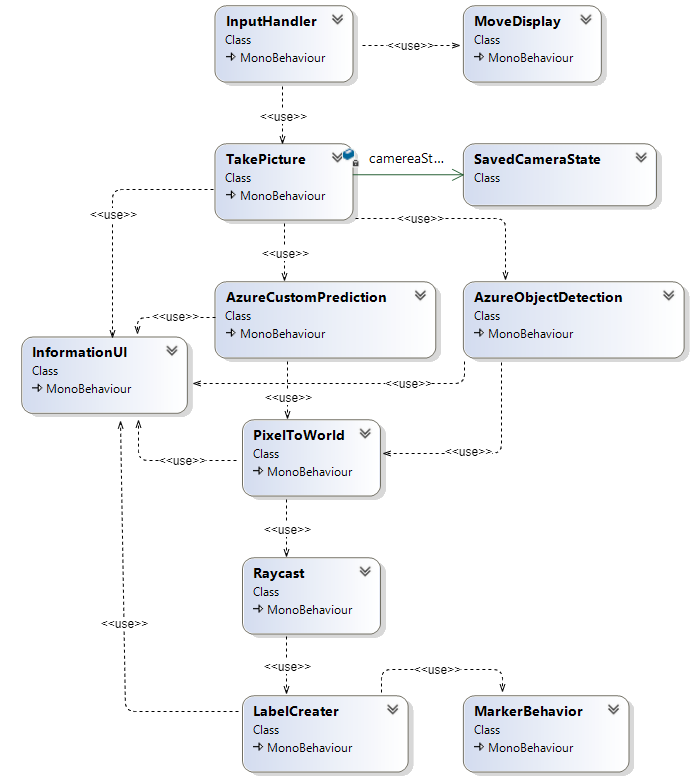
\includegraphics[width=1\textwidth]{images/klassendiagramm.png}
	\caption[Klassendiagramm der Skripts]{Klassendiagramme der Scripts}
	\label{dia:classdiagramm}
\end{figure}
 
Die Klassen InputHandler, MoveDisplay, LabelCreater, InformationUI und MarkerBehavior sind für die Interaktion mit dem dem Nutzer zuständig. 

TakePicture, SavedCameraState, AzureCustomPredicton,AzureObjectDetection,PixelToWorld und Raycast führen das Erkennen von Objekten anhand eines aufgenommenen Fotos durch und bestimmt eine Position für das Objekt in der 3D Umgebung. Der Prozess wird durch den InputHandler gestartet. 

Wurde ein Objekt erkannt und eine Position auf dem Mesh der Umgebung bestimmt, wird der LabelCreater aufgerufen. Es erzeugt das Label mit dem entsprechenden Text.

MarkerBehavior ist eine Script, das jedes Label GameObject hat, das erzeugt wird. Über das MarkerBehavior kann der Schriftzug des Labels angepasst werden.

\subsection{Interaktion}

InputHandler verarbeitet den Input des Nutzers und startet entsprechende Aktionen durch die MoveDisplay und TakePicture Klassen. 
MLInput ist eine vorgefertigte Klasse von Magic Leap. Sie stellt Informationen über den Zustand des Controllers zur Verfügung. InputHandler überwacht den Controller und startet die Aktionen, wenn die entsprechende Taste gedrückt wurde.

\begin{itemize}
	\item Trigger: Objekt Erkennung starten mit TakePicture
	\item Home Button: UI Element mittig vor das Display setzten.
	\item Bumper: Labels verstecken
	\item Bumper halten: zuletzt erzeugten Label entfernen 
\end{itemize}

Das UI Element wird von InformationUI gesteuert. TakePicture nutzt InformationUI um das zuletzt aufgenommene Foto anzuzeigen. AzureCustomPrediction, Azure ObjectDetection und PixelToWorld dokumentieren ihre Arbeitsschritte mit dem UI Element und der LabelCreater lässt eine Liste aller Labels anzeigen, die in der Szene existieren. Siehe Abbildung \ref{img:ausgabe}.

%\begin{figure}[H]
%	\centering
%	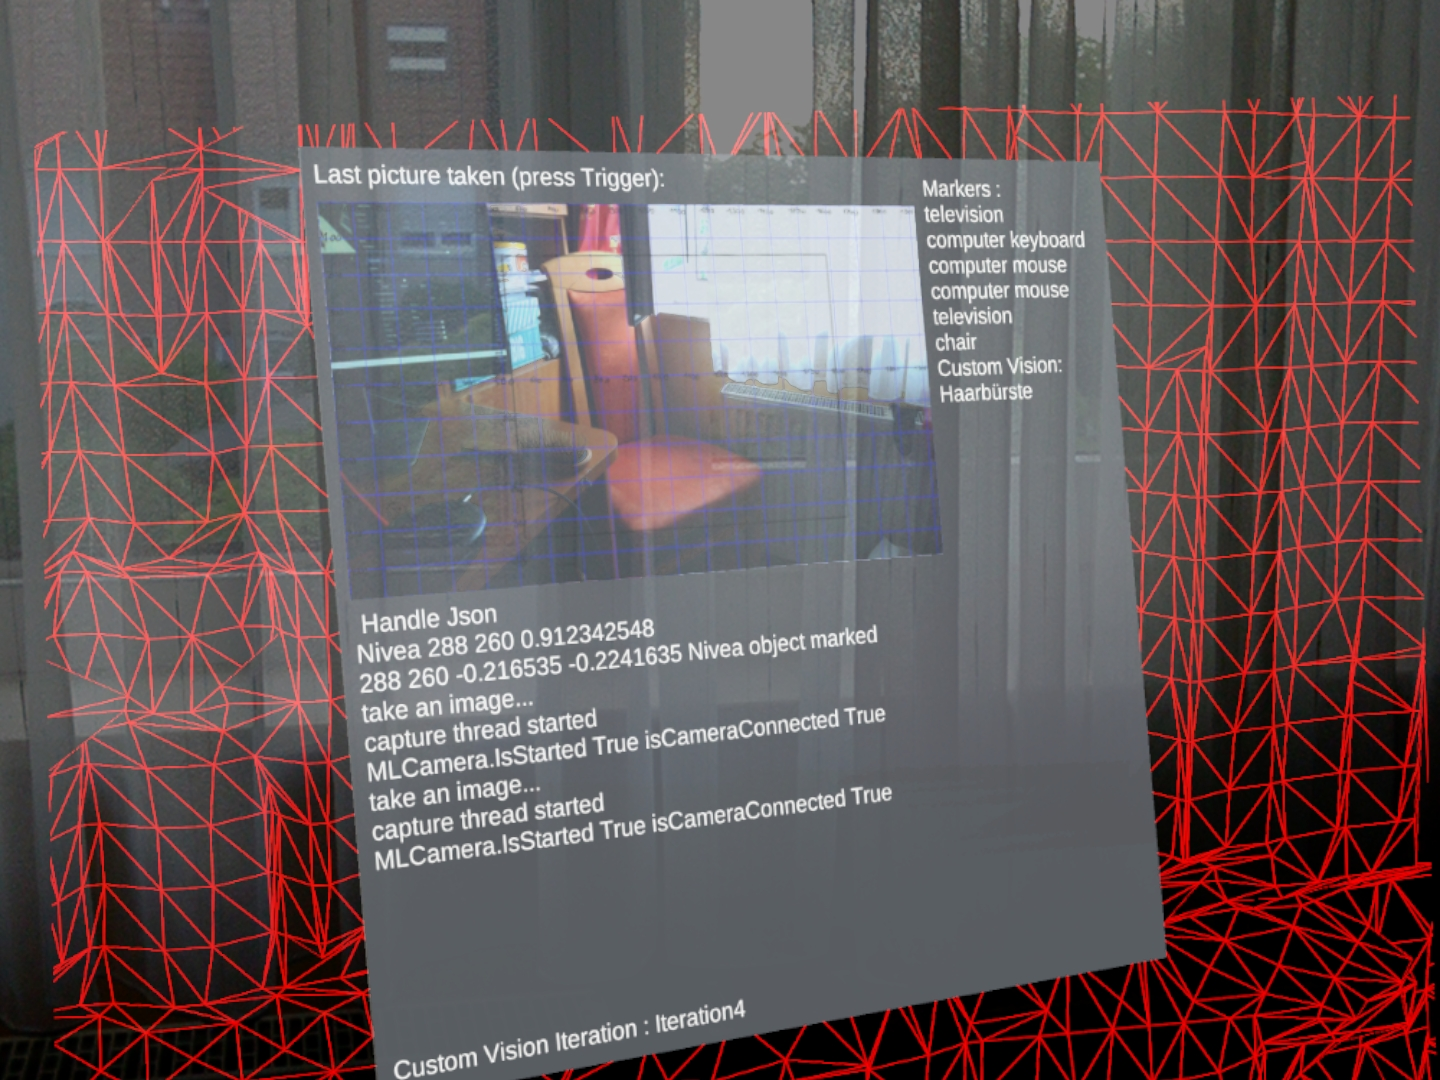
\includegraphics[width=1\textwidth]{images/ML_20200831_19.13.05.jpg}
%	\caption[]{UI Element}
%	\label{image:UIElement}
%\end{figure}

Der LabelCreater ist für das Erstellen der Labels verantwortlich und sorgt dafür, dass die Labels für den Nutzer lesbar sind.
Dafür werden die Labels in Richtung der Kamera ausgerichtet und mitgeführt.
Des Weiteren kann der LabelCreater Labels verstecken und entfernen.

Neben dem UI Element und den Labels wird auch ein Mesh angezeigt, das die Spatial Map der Umgebung wiedergibt. Das Spatial Mapping wird von Lumin OS durchgeführt und das Mesh wird durch die MLSpatialMapper Klasse von MagicLeap erzeugt. Siehe Abbildung \ref{img:ausgabe}.

\begin{figure}[H]
	\centering
	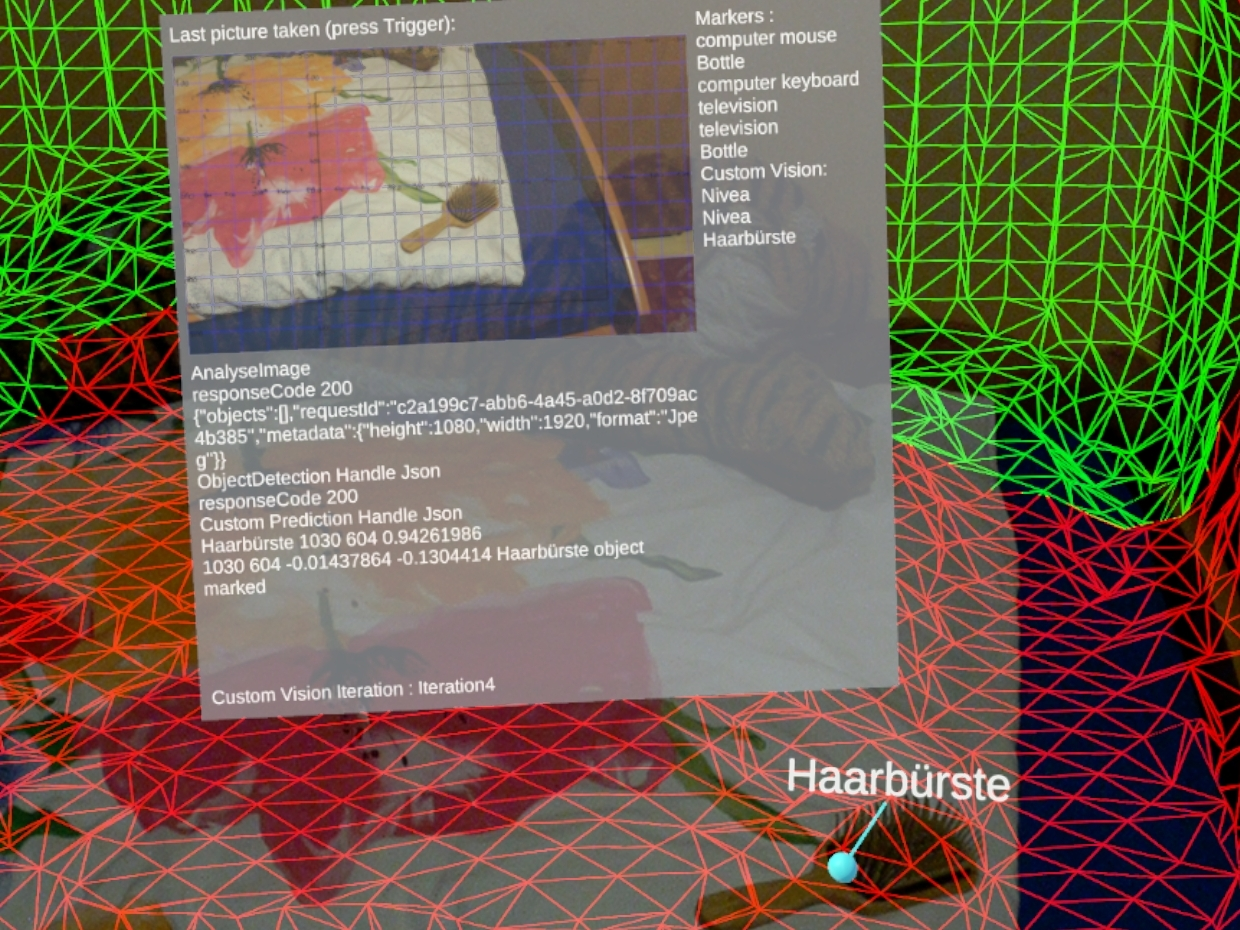
\includegraphics[width=0.9\textwidth]{images/ML_20201004_19.09.17_2.jpg}
	\caption[UI Ausgabe in der Szene]{Ausgabe}
	\label{img:ausgabe}
\end{figure}


\subsection{Implementierung der Objekt Erkennung}

Im Folgenden werden die Scripts besprochen, welche für die Objekterkennung zuständig sind.

\subsection{Ein Foto aufnehmen}

%\begin{figure}[H]
%	\centering
%	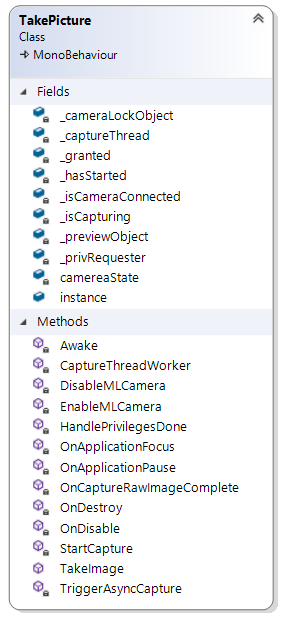
\includegraphics[width=0.4\textwidth]{images/dia_takepicture.PNG}
%	\caption[]{Klassendiagramm TakePicture}
%	\label{dia:takepicture}
%\end{figure} remake this image

Das Script TakePicture implementiert das Aufnehmen eines Fotos. Dabei wird MLCamera von MagicLeap genutzt, um die Kamera der Magic Leap Brille anzusteuern. Wenn die Applikation gestartet wird, stellt dieses Script sicher, das die Applikation die benötigte Permission hat die Kamera zu nutzen. Danach verbindet sich das Script über MLKamera mit der Kamera-Ressource. 
Die Kamera-Ressouce wird wieder abgegeben, wenn die Applikation terminiert oder pausiert wird.

Wenn die Methode TakeImage aufgerufen wird, startet der Prozess der Objekterkennung.
Das Aufnehmen der Fotos geschieht asynchron. Für jedes Foto wird ein Thread erzeugt, in dem MLCamera ein Foto aufnimmt. In diesem Thread wird zusätzlich die aktuelle Position der Unity Kamera als SavedCameraState gespeichert.

Die Methode OnCaptureRawImageComplete wird von MLCamera aufgerufen, wenn das Foto fertig ist. Die Daten des Bildes und der SavedCameraState werden, an die Scripts AzureObjectDetection und AzureCustomPrediction, weitergegeben. Dort wird die Analyse der Bilder gestartet. 

\subsubsection{Object Detection}

\begin{figure}[H]
	\centering
	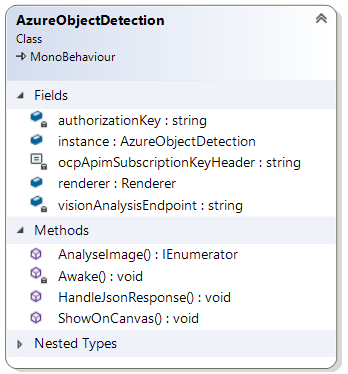
\includegraphics[width=0.5\textwidth]{images/dia_azureobjectdetection.PNG}
	\caption[Klassendiagramm von AzureObjectDetection]{Klassendiagramm von AzureObjectDetection}
	\label{dia:azureobjectdetection}
\end{figure}

In der Methode AnalyseImage von AzureObjectDetection wird ein Web Request zusammengestellt, um die Azure REST-API anzufragen. Der Request enthält eine Authentifizierung für die API und das zu analysierende Foto. %Siehe Abbildung \ref{dia:azureobjectdetection}.

Der Webrequest wird verschickt und auf die Antwort gewartet. Wenn die Antwort eintrifft, wird anhand des ResponseCodes geprüft, ob es bei dem Request einen Fehler gab. Beispielsweise kann die Internetverbindung gestört sein oder die Authentifizierung abgelehnt werden.
Wenn es keinen Fehler gab, wurde eine Json-Datei bei der Antwort mitgeschickt. Darin wird für jedes gefundene Objekt auf dem Foto eine Bezeichnung (Klasse) und eine Bounding Box angegeben. 

Die Json-Datei wird in HandleJsonResponse verarbeitet. Für den erwarteten Aufbau der Datei wurden drei Klassen geschrieben. Der Json String wird mit JsonUtility in ein DetectionResponse Object umgewandelt. Dabei werden alle gefundenen Foto-Objekte in einer Liste von DetectedObjects abgelegt. Siehe Abbildung \ref{dia:jsonClasses}. \citep{fromjson}

\begin{figure}[H]
	\centering
	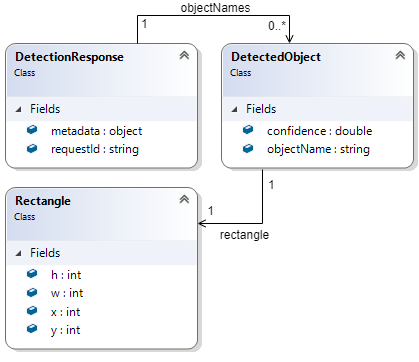
\includegraphics[width=0.6\textwidth]{images/dia_json.PNG}
	\caption[Klassendiagramm für Json umwandelung]{Klassendiagramm für die umwandeln der Json Datei in Objekte.}
	\label{dia:jsonClasses}
\end{figure}

Die gefundenen Objekte sollen im 3D Raum mit einem Label gekennzeichnet werden. 
Dafür wird für jedes DetectedObject die Methode Cast von der Klasse PixelToWorld aufgerufen. Der Methode wird der Mittelpunkt der BoundingBox als u,v Foto-Koordinaten für das DetectedObject übergeben. Siehe Abbildung \ref{code:handlejson}.

\begin{figure}[H]
	\centering
	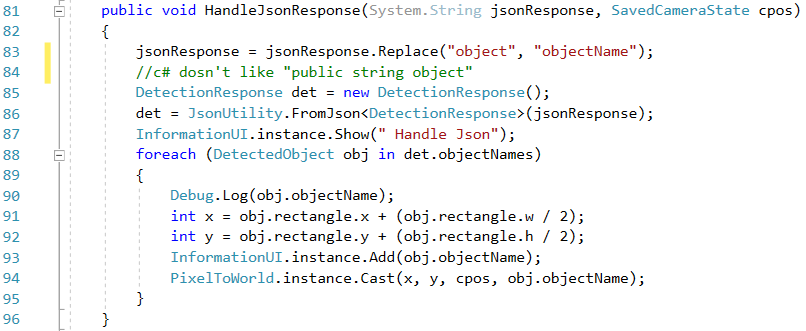
\includegraphics[width=1\textwidth]{images/code_handleJson.PNG}
	\caption[Quellcode Umwandelung der Json Datei in Objekte]{Quellcode Umwandeln der Json Datei in Objekte.}
	\label{code:handlejson}
\end{figure}

\subsubsection{Von dem Foto zum 3D Raum}

\begin{figure}[H]
	\centering
	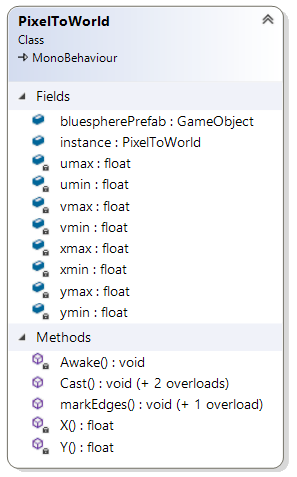
\includegraphics[width=0.45\textwidth]{images/dia_pixeltoworld.PNG}
	\caption[Klassendiagramm von PixelToWorld]{Klassendiagramm von PixelToWorld}
	\label{dia:pixeltoworld}
\end{figure}

Ein gefundenes Foto-Objekt soll in der 3D Abbildung der realen Welt lokalisiert werden. Dafür nutzt die Methode Cast die u,v Foto-Koordinaten des Objekts und einen SavedCameraState. Der SavedCameraState beschreibt die Position der Unity Kamera zu dem Zeitpunkt als das Foto aufgenommen wurde. SavedCameraState beinhaltete die cameraToWorldMatrix und den Ursprung der Kamera.

Das Foto kann mit dem Display und somit mit der Clipping Plane der Hauptkamera approximiert werden.
Die u,v Foto-Koordinaten werden zunächst in x,y,z Koordinaten in dem Camera Space umgewandelt. Der z Anteil gibt die Entfernung von dem Ursprung der Kamera in Blickrichtung an. Dabei befinden sich Punkte mit einer Entfernung von 0.4 Einheiten auf der Clipping Plane. In dem Camera Space mit z = -0.4 angegeben. 

Die x und y Dimensionen beschreiben die Achsen, die horizontal und vertikal zur Clipping Plane verlaufen. Mit dem festgelegten z = -0.4, kann jeder Punkt auf der Clipping Plane durch x und y angegeben werden. Dazu gehören auch Punkte die außerhalb des View Frustum liegen.

Es wurden Werte für x und y ausprobiert, mit denen die Ränder des Fotos auf der Clipping Plane angegeben werden können. Dabei wurde auf die unterschiedlichen Seitenverhältnisse des Fotos und des Displays geachtet. Darüber hinaus ist der Bildausschnitt des Displays kleiner. Daher liegen die Ränder des Fotos außerhalb des View Frustum. 

Sind diese x und y Werte bekannt, ergibt sich für die Achsen jeweils ein Intervall, die kombiniert alle Foto-Koordinaten auf die Clipping Plane abbilden können. Die Intervall lauten: [-0.2949,0.2295] für x und [0.1546,-0.1507] für y. Mit den Intervallen wird die Position und Skalierung des Fotos in Relation zu dem Display - und der Hauptkamera - berücksichtigt. Siehe Kapitel \ref{section:devpixeltoworld} für die Entwickelung der Cast Methode und die Ermittlung der Intervallwerte.

Es werden zwei lineare Funktionen aufgestellt:
\begin{itemize}
	\item Die Funktion X bildet das Intervall für u [0,1920] auf das Intervall für x [-0.2949,0.2295] ab.
	\item Die Funktion Y bildet das Intervall für v [0,1080] auf das Intervall für y [0.1546,-0.1507] ab.
\end{itemize}
Siehe Abbildung \ref{code:uvtoxy}.
\begin{figure}[H]
	\centering
	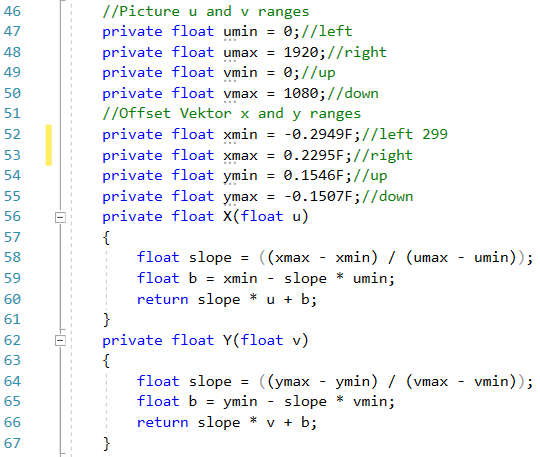
\includegraphics[width=0.6\textwidth]{images/code_uv_to_xy_scale.PNG}
	\caption[Quellcode der Funktionen X und Y]{Quellcode der Funktionen X und Y}
	\label{code:uvtoxy}
\end{figure}

Mit den Funktionen wird eine Position im Camera Space, auf der Clipping Plane, für u,v berechnet. Diese Position wird dann, mithilfe der cameraToWorldMatrix des SavedCameraState, in eine Position p des globalen Koordinatensystem umgewandelt. Damit wird die Position und Rotation der Kamera - und somit des Fotos - in der 3D Szene berücksichtigt. Siehe Abbildung \ref{code:castmethod}.

\begin{figure}[H]
	\centering
	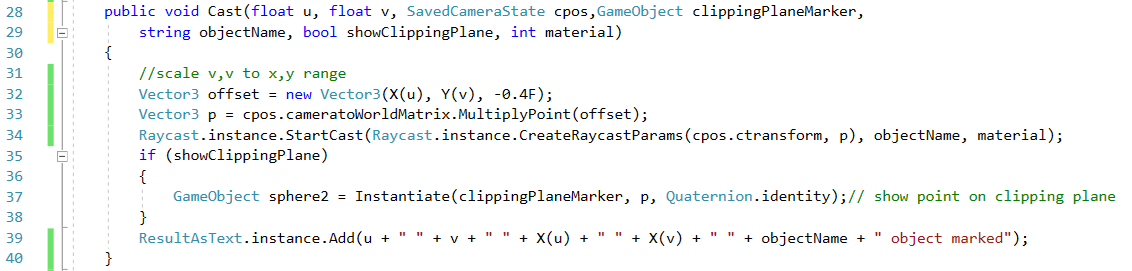
\includegraphics[width=1.2\textwidth]{images/code_cast_method.PNG}
	\caption[Quellcode der Cast Methode]{Quellcode der Cast Methode}
	\label{code:castmethod}
\end{figure}
\subsubsection{Raycast}

\begin{figure}[H]
	\centering
	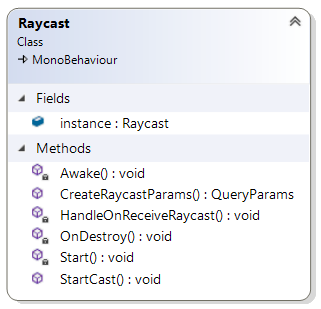
\includegraphics[width=0.45\textwidth]{images/dia_raycast.PNG}
	\caption[Klassendiagramm von Raycast]{Klassendiagramm von Raycast}
	\label{dia:raycast}
\end{figure}

Als Nächstes wird ein Raycast durch den Ursprung der Kamera und die Position p gesendet. MLRaycast wird genutzt, um einen Schnittpunkt mit der Rekonstitution der Welt von Lumin OS zu bestimmen. Die Stelle, die der Raycast trifft beschreibt die Position des DetectedObject im 3D Raum.

Für den MLRaycast werden zwei Parameter benötigt:
\begin{itemize}
	\item Ein QueryParams Objekt, das Ursprung und Richtung für den Raycast beinhaltet.
	\begin{itemize}
		\item Ursprung: Kamera-Ursprung aus SavedCameraState
		\item Richtung: Richtungsvektor von dem Kamera-Ursprung zu der Position p
	\end{itemize}
	\item Eine Methode die aufgerufen wird, wenn der Raycast fertig ist. 
	\begin{itemize}
		\item Callback Methode: HandleOnRecieveRaycast
	\end{itemize}
\end{itemize}

Siehe Abbildung \ref{code:raycastparams}.

\begin{figure}[H]
	\centering
	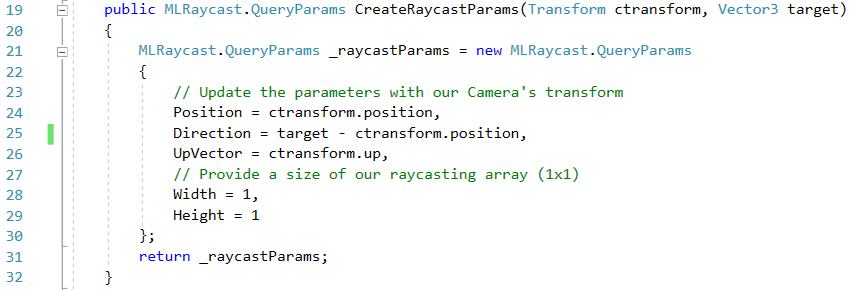
\includegraphics[width=1\textwidth]{images/code_raycastparams.PNG}
	\caption[Quellcode Erzeugung der Raycast Parameter]{Quellcode Erzeugung der Raycast Parameter}
	\label{code:raycastparams}
\end{figure}

Wenn der Raycast fertig ist, wird die Methode HandleOnRecieveRaycast aufgerufen. Der Parameter point beinhaltet dabei die getroffene Stelle der AR Umgebung.
Diese wird an die Methode CreateMarker von der Klasse LabelCreater weitergegeben.

\subsubsection{LabelCreater}

%\begin{figure}
%	\centering
%	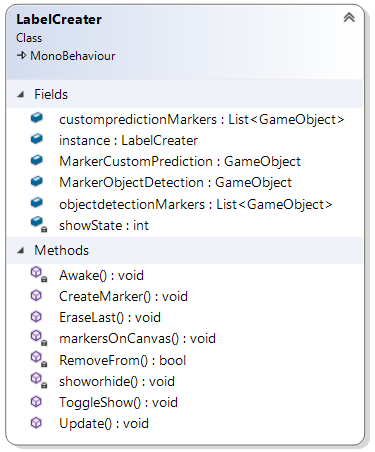
\includegraphics[width=0.5\textwidth]{images/dia_labelcreater.PNG}
%	\caption[]{Markierungen in der Welt}
%	\label{dia:labelcreater}
%\end{figure}

CreateMarker erhält den Punkt point, der getroffen wurde und die Bezeichnung für das DetectedObject. An der Position von point wird ein Prefab GameObject instanziiert, das als Markierung für das DetectedObject in der 3D Umgebung dient.

Das Prefab besteht aus einer Kugel und einem Schriftzug, der den Namen des DetectedObject anzeigen soll. Dem neu instanziierten GameObject wird die Bezeichnung des DetectedObject als Schriftzug zugewiesen. Siehe Abbildung \ref{image:labels}.

\begin{figure}[H]
	\centering
	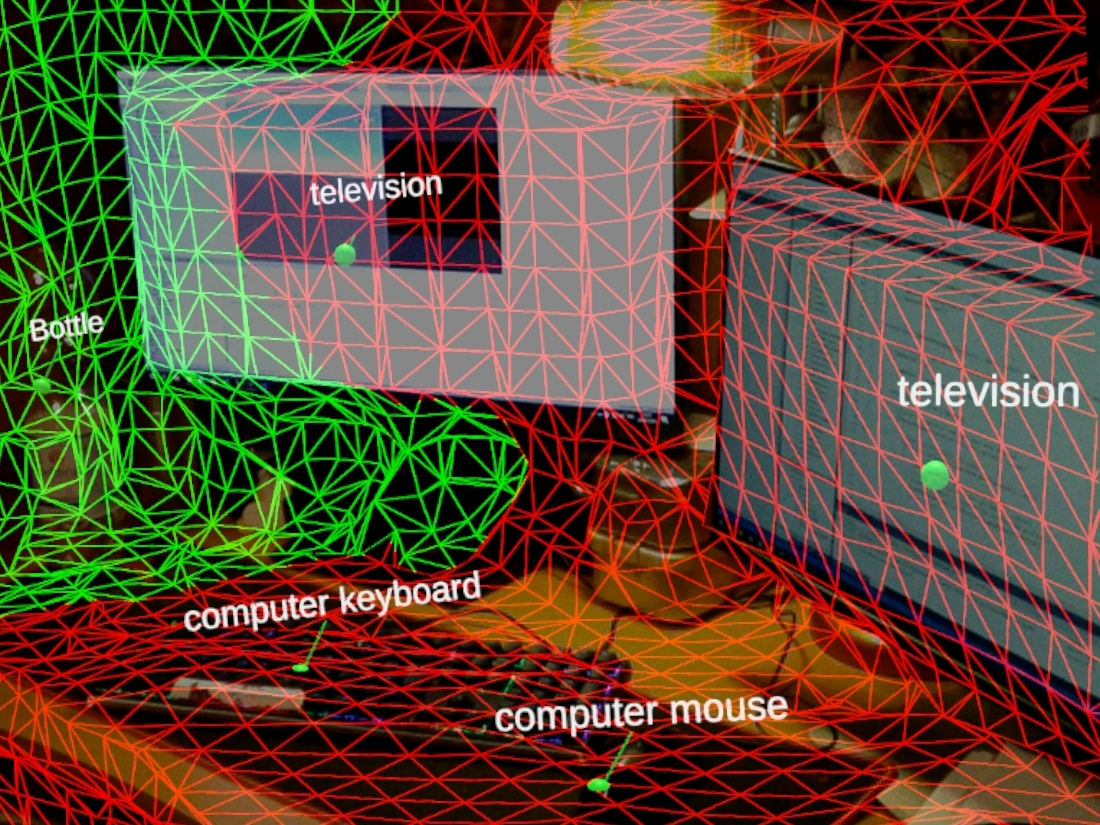
\includegraphics[width=0.8\textwidth]{images/ML_20201004_19.10.05_2.jpg}
	\caption[Labels in der Szene]{Labels in der Szene}
	\label{image:labels}
\end{figure}

Wenn ein Label nahe eines anderen Labels erzeugt werden soll, das denselben Schriftzug hat, wird davon ausgegangen, das ein Objekt der realen Welt erneut erkannt wurde. Daher wird kein neues Label erstellt, sondern das alte Label modifiziert.
Die Positionen an denen das Objekt in der Szene lokalisiert wurde, werden mit jeweils einer grauen Sphäre markiert und das Label wird in den Mittelpunkt der grauen Sphären gesetzt.
So  wird die Position des Objektes genauer, wenn es häufiger erkannt wurde. Siehe Abbildungen \ref{image:multi1} und \ref{image:multi2}.

\begin{figure}[H]
	\centering
	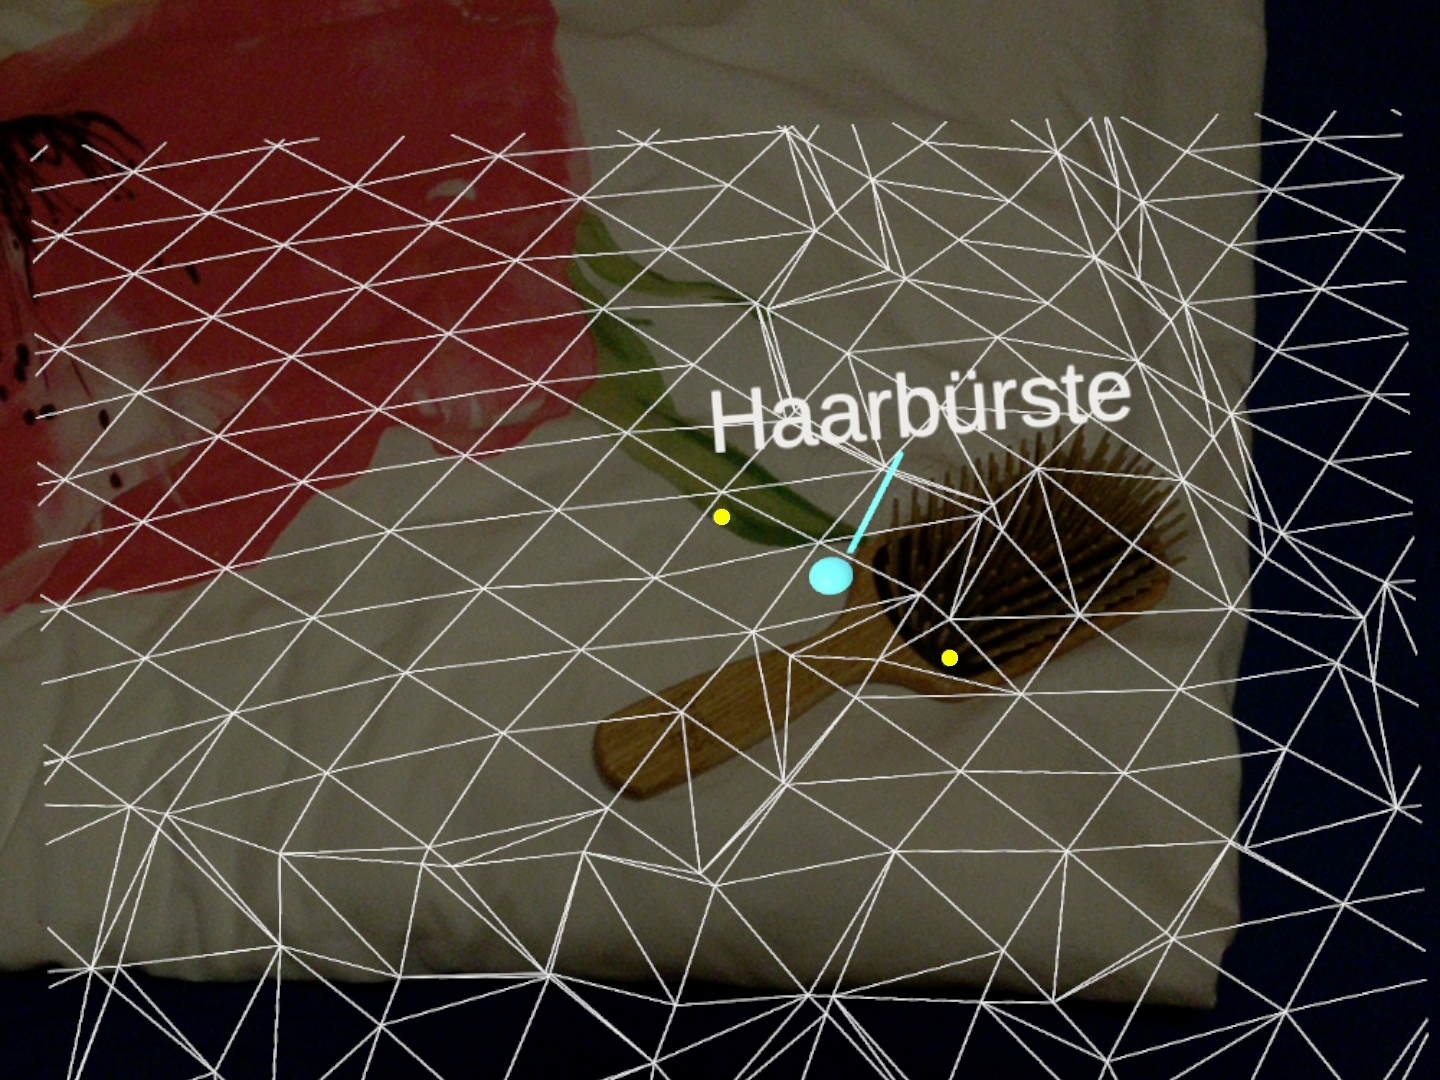
\includegraphics[width=0.7\textwidth]{images/ML_multi1.jpg}
	\caption[Haarbürste zwei mal Erkannt]{Haarbürste zwei mal Erkannt. Graue Sphären hier in gelb markiert.}
	\label{image:multi1}
\end{figure}


\begin{figure}[H]
	\centering
	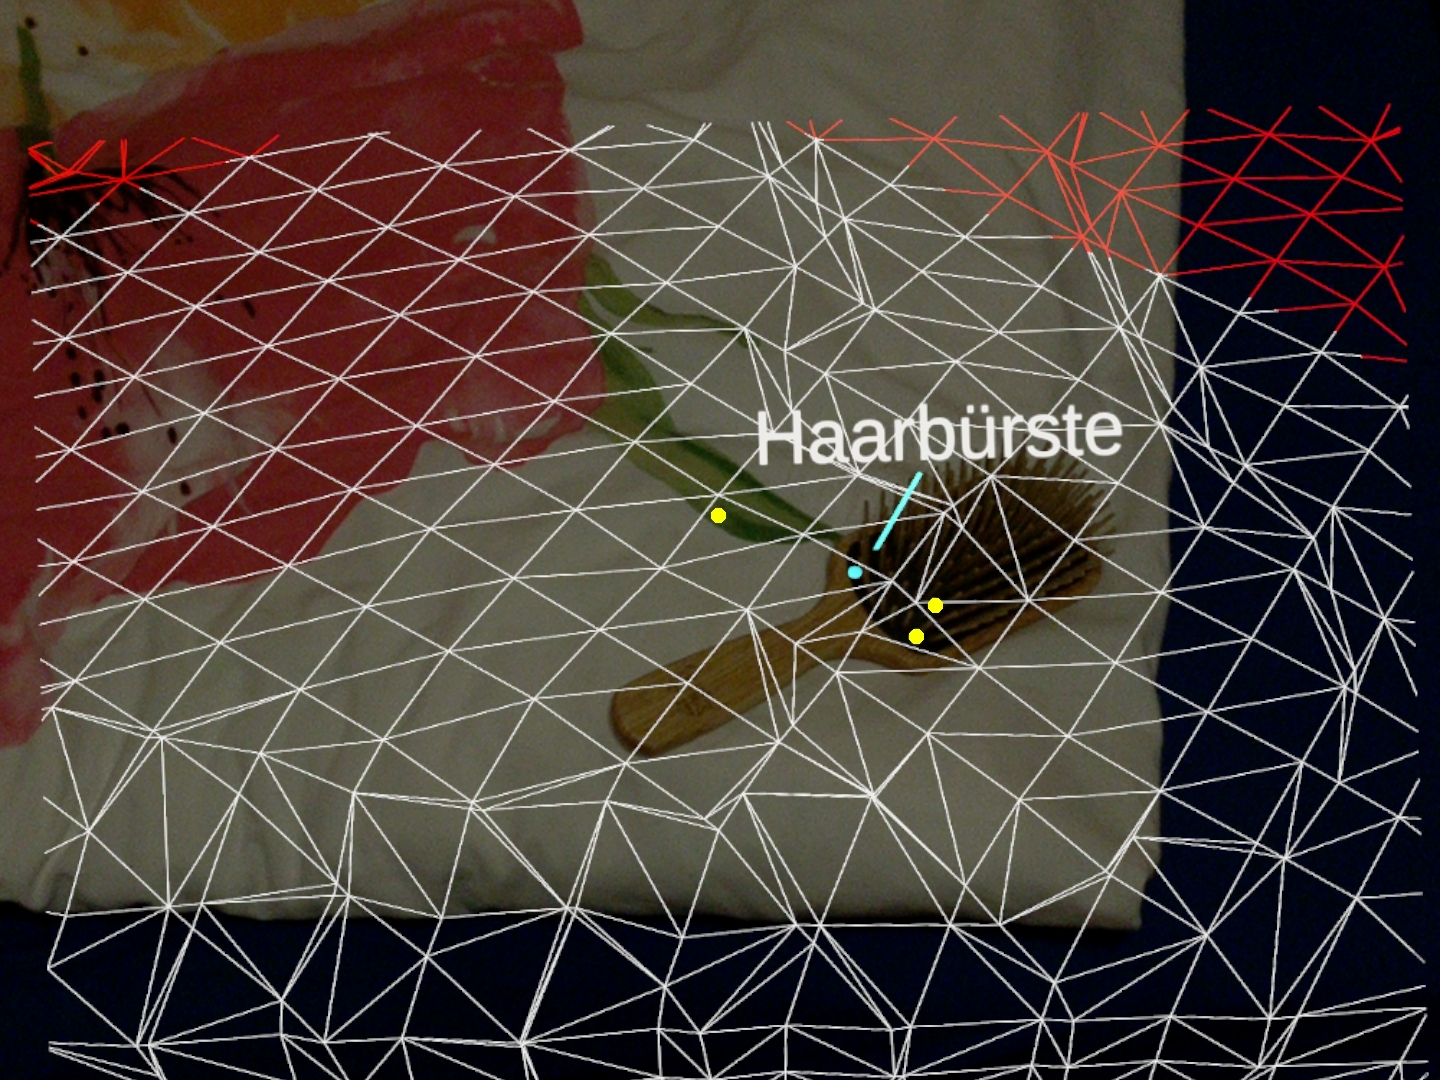
\includegraphics[width=0.7\textwidth]{images/ML_multi2.jpg}
	\caption[Haarbürste drei mal Erkannt]{Haarbürste drei mal Erkannt. Graue Sphären hier in gelb markiert.}
	\label{image:multi2}
\end{figure}

Die erzeugten Labels werden in den Listen MarkerCustomPredicton und MarkerObjectDetection gespeichert, je nachdem welcher Azure Service verwendet wurde. 
Zu jedem Frame der Applikation werden die Labels in den Listen zur Kamera hingedreht sodass sie rechtwinklig zur Kamera ausgerichtet sind. Als Resultat werden die Labels der Bewegung der Kamera nachgeführt. Solange das Label in dem View Frustum liegt, kann der Nutzer es lesen. Siehe Anhang \ref{appendix:blickwinkel}.

\subsubsection{Azure Custom Vision}

Neben der Bildanalyse mit Azure Object Detection wird auch Azure Custom Vision verwendet.
Die AI wurde über die Webseite trainiert.

Die Anfrage an den Service geschieht in der Klasse AzureCustomPrediction. Ähnlich wie bei AzureObjectDetection wird ein Webrequest erstellt mit einem Authorization Key und einem Foto. Die Anfragen an die beiden REST-APIs werden parallel in unterschiedlichen Threads erstellt und bearbeitet.

In der Antwort wird eine Json Datei zurückgeschickt, die die gefundenen Objekte angibt.
Da die Json Datei eine etwas anderes Format hat, wurde eine eigene HandleJsonResponse Methode dafür geschrieben.

Azure Custom Vision gibt für jedes Detected Object eine Probability an. Diese gibt das Vertrauen des Modells darin an, dass das Objekt korrekt erkannt wurde.

Es wurde ein Schwellwert definiert, der entscheidet wie hoch die Probability mindestens sein muss, um das Objekt zu akzeptieren und in der Szene zu markieren.

Für jedes akzeptierte Objekt wird die Methode Cast von PixelToWorld aufgerufen, um das Objekt in der realen Welt zu lokalisieren und zu markieren.

\paragraph{Das Trainieren}

Es wurde probiert das Custom Vision Modell auf drei unterschiedliche Objekte zu trainieren.
Dabei wurden vier Iterationen erstellt. 

Iteration 1:

Zunächst wurde probiert Tuben von Acrylfarbe zu erkennen. In der Nutzung dieser Iteration traten viele fehlerhaften Objekterkennungen auf. Es wurden Acrylfarben an Stellen erkannt, an denen es keine gab. Siehe Abbildung \ref{image:customVisionPaint}. 

\begin{figure}[H]
	\centering
	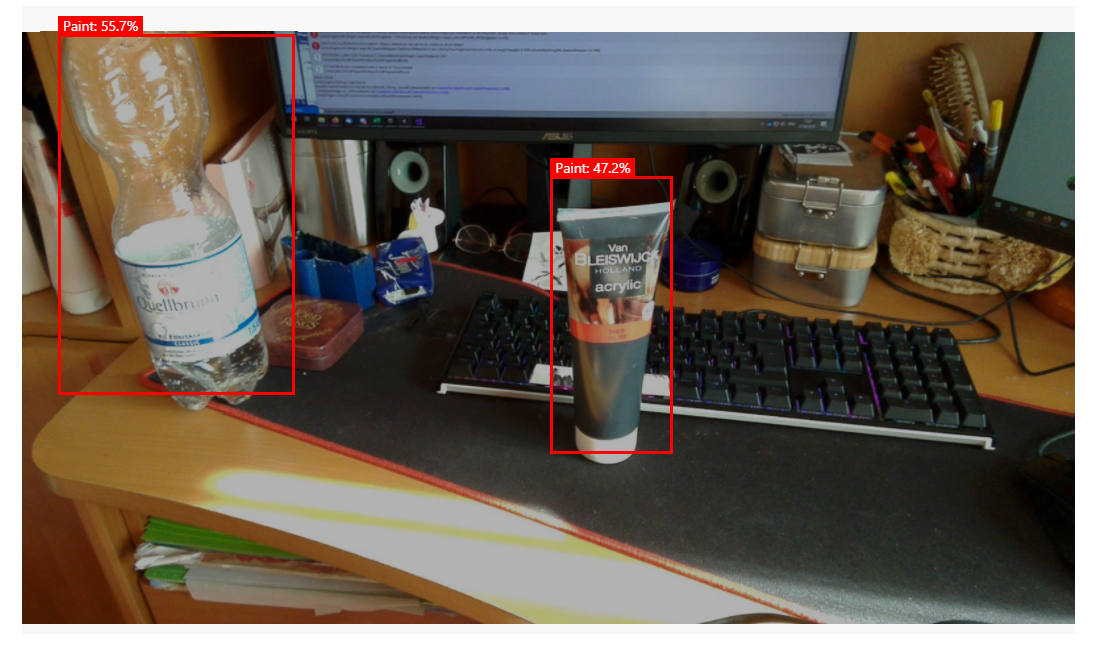
\includegraphics[width=1.0\textwidth]{images/customVisionPaint.PNG}
	\caption[Iteration 1 Analysebeispiel]{Iteration 1 Analysebeispiel. Eine Wasserflasche und eine Farbtube wurden beide als Farbtuben erkannt. Die Wasserflasche wurde mit einer Probability von 55.7 Prozent markiert, während die tatsächliche Farbtube eine Probability von 47.5 Prozent hat.}
	\label{image:customVisionPaint}
\end{figure}

Die Evaluierung des Modelles lautet: 66.7\% Precision, 66.7\% Recall, 89.7\% mean Average Precision.

\begin{itemize}
	\item Precision - die Wahrscheinlichkeit das ein gefundenes Objekt, tatsächlich der angegeben Klasse angehört. (Die Wahrscheinlichkeit das es kein false positive ist.)
	\item Recall - Aus einer Menge an Objekten die einer Klasse angehören, der Prozentsatz an Objekten, die das Modell korrekt lokalisieren und klassifizieren konnte.
	\item m.a.p (mean Average Precision) - Eine Gesamtwertung für die Evaluierung basierend auf Precision und Recall. 
\end{itemize}

\paragraph{Iteration 2}

In der zweiten Iteration wurde probiert, das Modell darauf zu trainieren, eine blaue Dose von Nivea Hautcreme zu erkennen. Die Form und Farbe der Dose ist sehr simpel, daher wurde davon ausgegangen, dass sie leichter zu erkennen ist. Die berechnete Prediction des Modells lag bei 80 Prozent. Wenn eine Nivea Dose erkannt wurde, ist das Modell sich zu 80 Prozent sicher, dass es sich tatsächlich um eine Nivea Dose handelt.

Die Evaluierung des Modells lautet: 80\% Precision, 100\% Recall, 100\% mean Average Precicion.
In einer Testphase konnte das Modell alle auf den Bildern erhaltenen Nivea Dosen zu erkennen (100\% Recall), es hat jedoch auch Objekte fälschlicherweise als Dosen markiert (80\% Precision).

Trotzdem wurden in vielen Fotos fälschlicherweise Nivea Dosen erkannt. 


\paragraph{Iteration 3}

In der dritten Iteration wurde versucht die vorherige Iteration zu verbessern. Es wurden ausgewählte Trainingsfotos entfernt, die die Dose von einem seitlichen Winkel zeigten. Die Erwartung war, dass die Detektion der Dose aus dem Blickwinkel von oben konsistenter wird. Zusätzlich wurden mehr Fotos von der Dose auf unterschiedlich gefärbten und gemusterten Untergründen hinzugefügt. 

Die Precision sank auf 75 Prozent.

Die Evaluierung des Modells lautet: 75\% Precision, 100\% Recall, 100\% mean Average Precicion.
Dises Modell hat in der Testphase häufiger Objekte fälschlicherweise als Dosen markiert.

\paragraph{Iteration 4}

In der vierten Iteration wurden zwei Fotos von der Nivea Dose entfernt, was die Precision auf 100 Prozent steigen ließ. In der Umsetzung mit der Magic Leap Anwendung wurden trotzdem häufig Objekte fälschlicherweise als Nivea Dose markiert.

Neben der Dose wurde diese Iteration darauf trainiert eine bestimmte Holzhaarbürste zu erkennen. Aufgrund von dem komplexeren, und markanten Aussehen der Bürste wurde davon ausgegangen, das die Bürste besser von anderen Objekte zu unterschieden ist. 
Die Bürste wurde nur mit den Borsten nach oben fotografiert.

Die Evaluierung des Modells lautet: 100\% Precision, 100\% Recall, 100\% mean Average Precicion.

Objekte die mit einer Wahrscheinlichkeit von über 80 Prozent als Haarbürsten markiert wurden, waren in der Anwendung tatsächlich Haarbürsten. Durch das Setzen dieses Schwellenwertes wurden keine Objekte fälschlicherweise als Haarbürste erkannt. Siehe Abbildung \ref{img:it4}.

\begin{figure}[H]
	\centering
	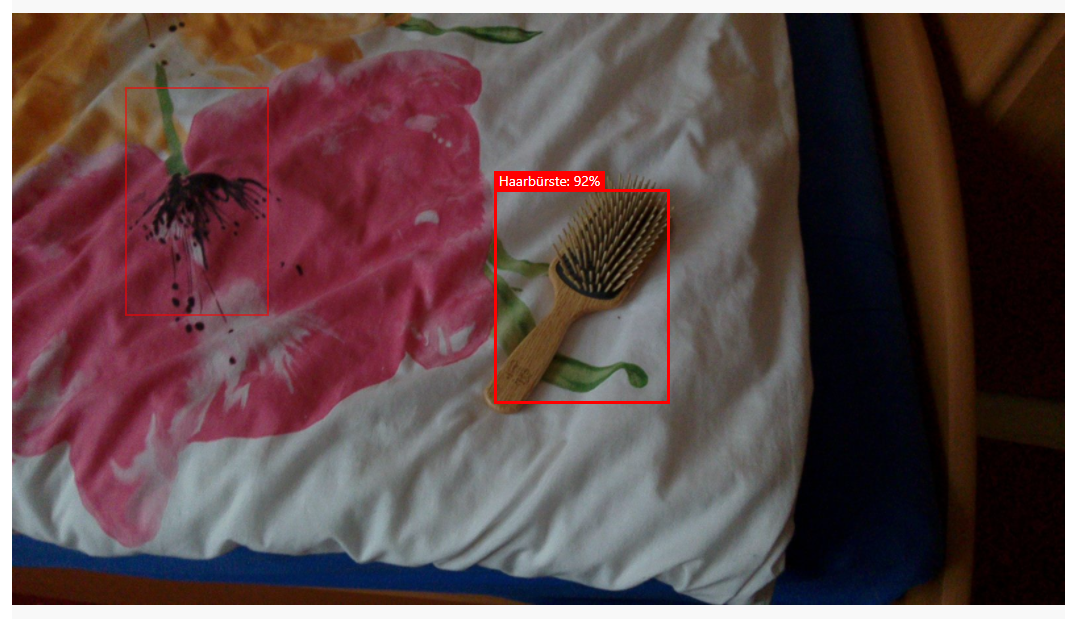
\includegraphics[width=0.8\textwidth]{images/it4notpretty.png}
	\caption[Iteration 4 Analysebeispiel]{Iteration 4 Analysebeispiel. Die Tatsächliche Haarbürste wurde mit einer Probability von 92 Prozent erkannt. Eine Blume auf einer Decke wurde zu 71,3 Prozent als Haarbürste erkannt.}
	\label{img:it4}
\end{figure}

Wenn die Haarbürste in dem Foto kleiner abgebildet ist, sind die Probability so weit, das die Bürste sich nicht mehr anhand des Schwellenwert von anderen Objekten unterscheiden lässt.

\begin{figure}[H]
	\centering
	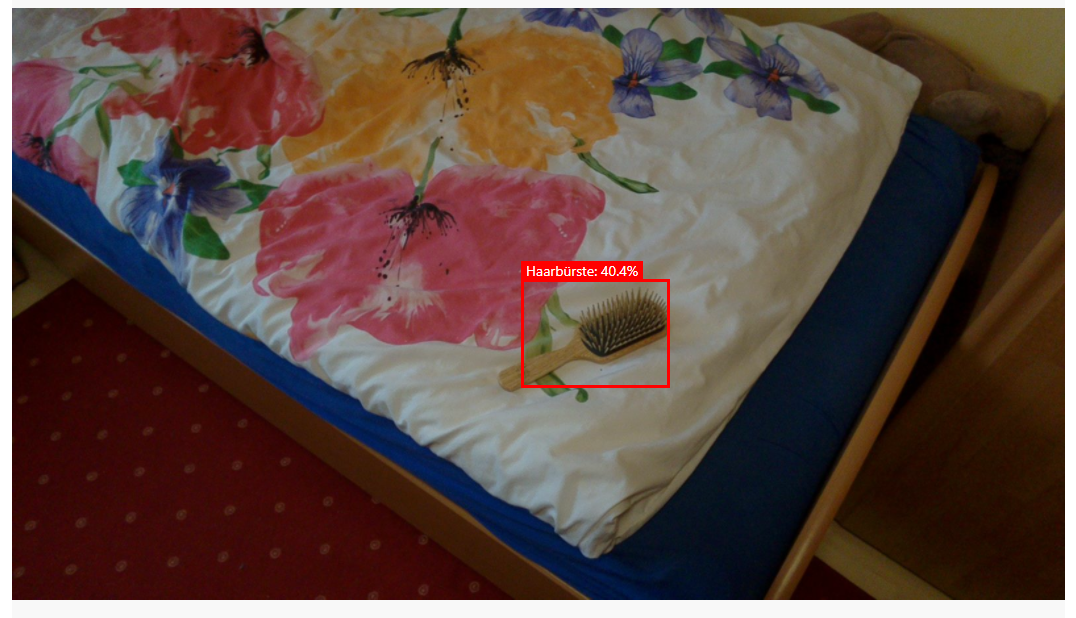
\includegraphics[width=0.8\textwidth]{images/it4notpretty2.png}
	\caption[Iteration 4 zweites Analysebeispiel]{Iteration 4 Analysebeispiel. Die Tatsächliche Haarbürste wurde mit einer Probability von 40,4 Prozent erkannt.}
	\label{img:it4}
\end{figure}
\paragraph{Iteration 5}

Iteration 5 ist eine Variation von Iteration 4. Die Objekterkennung der Nivea Dose entfernt. Die Iteration ist nur noch darauf trainiert die Haarbürste zu erkennen. 

Die Evaluierung des Modells lautet: 100\% Precision, 100\% Recall, 100\% mean Average Precicion.

\paragraph{Iteration 6}

In der Iteration 6 wurde die Erkennung der Haarbürste verbessert. Den Empfehlungen von Azure folgend, wurde die Menge an Trainingsbildern auf 51 erhöht. Auf den Trainingsbildern ist die Haarbürste teilweise recht klein zu sehen. Siehe Anhang \ref{appendix:it4train}. Dieser Iteration wurde eine Stunde Zeit gelassen, um das Training durchzuführen. Vorherige Iteration hatten ca. 10 Minuten.

Die Evaluierung des Modells lautet: 100\% Precision, 100\% Recall, 100\% mean Average Precicion.

Haarbürsten, die kleiner in einem Foto sind, konnten von dieser Iteration erkannt werden. Siehe Abbildung \ref{img:it6}. Mit den vorherigen Iterationen war das nicht möglich. Die Haarbürste musste immer recht groß im Bild sein. 

In den Bildern, die von Iteration 6 analysiert wurden, waren alle Objekte, die das Model mit einer Wahrscheinlichkeit von über 50 Prozent als Haarbürste markiert hatte, tatsächlich Haarbürsten.

\begin{figure}[H]
	\centering
	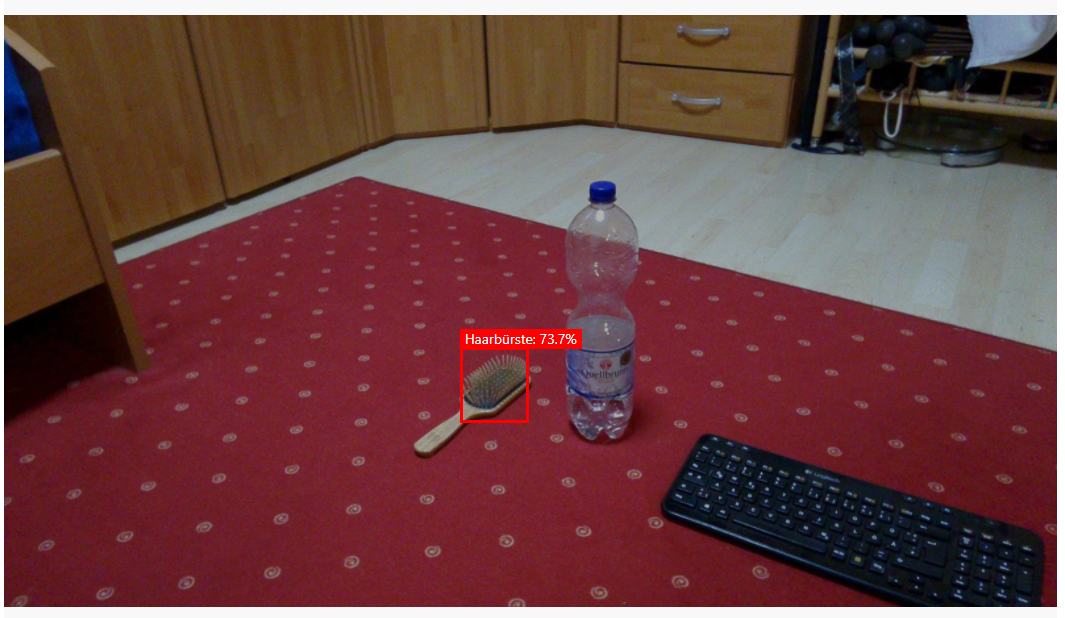
\includegraphics[width=0.8\textwidth]{images/it6pretty.png}
	\caption[Iteration 6 Analysebeispiel]{Iteration 6 Analysebeispiel. Haarbürste mit einer Probability von 73,7 Prozent erkannt.}
	\label{img:it6}
\end{figure}


\subsection{Entwicklung der Foto-Repräsentation}
\label{section:devpixeltoworld}

Um die u,v Foto-Koordinate eines gefundenen Objektes auf der Clipping Plane der Kamera zu lokalisieren, wurden ein paar Herangehensweisen ausprobiert.

Das Ziel ist das Setzten einer Markierung in den 3D Raum, basierend auf den Foto-Koordinaten. Das Foto beinhaltet keine Information über die Entfernung zu dem Objekt. Dafür muss ein Raycast durchgeführt werden. 

Mit einer Repräsentation des Fotos in dem 3D Raum ist es möglich diesen Raycast durchzuführen. 
Dazu muss das Foto nicht tatsächlich in dem 3D Raum vorhanden sein. Es muss jedoch mit dem Input der Foto-Koordinaten ein Output der x,y,z-Koordinaten in dem 3D Raum erzeugt werden, mit dem der Raycast durchgeführt werden kann.

Die Position des Fotos hängt mit der Kamera zusammen, daher kann das Foto durch den Camera Space simuliert werden. Als erstes wurde probiert ein Sphären-Objekt an eine gezielte Koordinate des Camera Space zu bewegen. 

% make pretty after this
Wenn die Kamera am Ursprung des globalen Koordinatensystem liegt und eine neutrale Rotation hat, stimmt der Camera Space mit dem globalen Koordinatensystem überein. Die Sphäre wurde in der Szene per Hand bewegt um markante Koordinaten des Camera Space abzulesen. Siehe Abbildung \ref{illustration:speretest}.

\begin{figure}[H]
	\centering
	\includegraphics[width=0.7\textwidth]{images/sphärenTest.PNG}
	\caption[Ränder der Near Clipping Plane in Unity finden]{Die blaue Sphäre liegt auf dem linken Rand der Clipping Plane.}
	\label{illustration:speretest}
\end{figure}

Dabei wurden folgende Camera Space Koordinaten gefunden:
\begin{itemize}
	\item Near Clipping Plane bei z = -0.37
	\item linker Rand bei x = -0.153
	\item rechter Rand bei x = 0.153
	\item oberer Rand bei y = 0.1147
	\item unterer Rand bei y = -0.1147
\end{itemize}

Die x und y Koordinaten hängen von den u,v Koordinaten des Fotos ab. Es wurden lineare Funktionen aufgestellt um u,v auf x,y abzubilden. Diese Abbildung dient als Repräsentation des Fotos im 3D Raum, unter Berücksichtigung der Position und Skalierung des Fotos im Verhältnis zu der Kamera.

Dann wurde getestet wie genau DetectedObjects in der AR Umgebung lokalisiert werden. Es wurden testweise Fotos aufgenommen, analysiert und die DetectedObjects markiert. Die entstandenen Markierungen lagen in Sichtfeld, jedoch nicht an den erwarteten Stellen. 

Um dem Problem auf den Grund zu gehen, wurde ein UI Objekt erstellt, das ein aufgenommenes Foto während der Laufzeit anzeigt.
Das Foto wurde dann mit dem Display verglichen. Dabei fiel auf, das sie ein unterschiedliches Seitenverhältnis haben und das Display einen kleinen Bildausschnitt zeigt.  

Es gibt zwei Möglichkeiten die Unterschiede zwischen Foto und Display auszugleichen. Entweder wird das Foto auf das Display zugeschnitten oder das gesamte Foto wird verwendet. Im zweiten Fall würden auch Objekte erkannt, die außerhalb des Sichtfeldes liegen.
Es wurde die Entscheidung getroffen das Foto zuzuschneiden. Damit gibt es ein besseres Feedback für den Nutzer, wenn ein Objekt gefunden wurde. 

Das Zuschneiden wurde realisiert, indem die Intervalle für u und v der Abbildungsfunktionen stärker eingegrenzt wurden. Alle Objekte die außerhalb der Intervalle liegen werden ignoriert. Um die Intervalle zu bestimmen wurde dem Fotoanzeige-UI-Element ein Gitter hinzugefügt. Mit dem Gitter kann die u,v Position von beliebigen Stellen des Fotos abgelesen werden. 
Durch Aufnehmen von Fotos und Vergleichen mit dem Sichtfeld des Displays wurde abgelesen, bei welcher u,v Position des Fotos die Ecken des Displays zu finden sind. Die Intervalle wurden dem entsprechend eingegrenzt. 

Mit den durchführten Veränderungen der Intervalle konnten DetectedObjects korrekt in der Umgebung lokalisiert werden. Jedoch wurden sehr häufig Objekte nicht markiert, obwohl sie im Sichtfeld des Nutzers lagen, weil deren Mittelpunkt außerhalb eines Intervalls lag.

Daher wurde entschieden die zweite Möglichkeit zu implementieren und das gesamte Foto zu verwenden und Objekte auch zu markieren, wenn sie komplett außerhalb des Sichtfeldes liegen. 
Dafür wurden die Intervalle für u und v wieder auf die ursprünglichen Werte - [0,1920] und [0,1080] - gesetzt. Die Intervalle für x und y mussten vergrößert werden.

Um die x und y Intervalle bestimmen zu können, wurde das Fotoanzeige-UI-Element Parallel zu der ClippingPlane gelegt. Das Element folgt den Bewegungen der Kamera und liegt möglichst nah an der Near Clipping Plane. Das Display der Magic Leap Brille zeigt selbst solide Objekte leicht durchsichtig an. Das wurde genutzt, um Fotos aufzunehmen, mit dem UI Element anzuzeigen und mit der realen Welt zu vergleichen. Durch Ausprobieren wurde das UI Element so skaliert und verschoben, dass das angezeigte Foto mit der realen Welt soweit wie möglich übereinstimmt. Siehe Abbildungen \ref{illustration:canvasinsourface} und \ref{illustration:canvasinsourfacetodown}.

\begin{figure}[H]
	\centering
	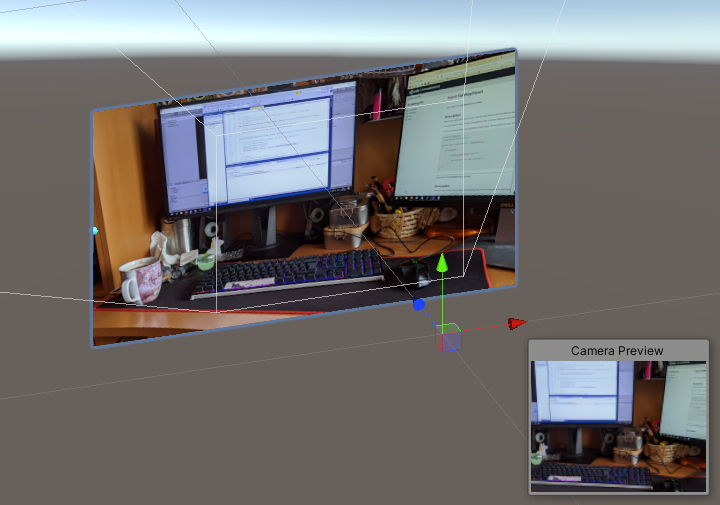
\includegraphics[width=0.8\textwidth]{images/canvasinyourface.PNG}
	\caption[Ränder des Foto-Anzeige-Elements finden]{Das aufgenommene Foto füllt das gesamte Display aus, wenn es angezeigt wird. Die blaue Sphäre liegt auf dem linken Rand des Foto-Anzeige-Elementes.}
	\label{illustration:canvasinsourface}
\end{figure}

\begin{figure}[H]
	\centering
	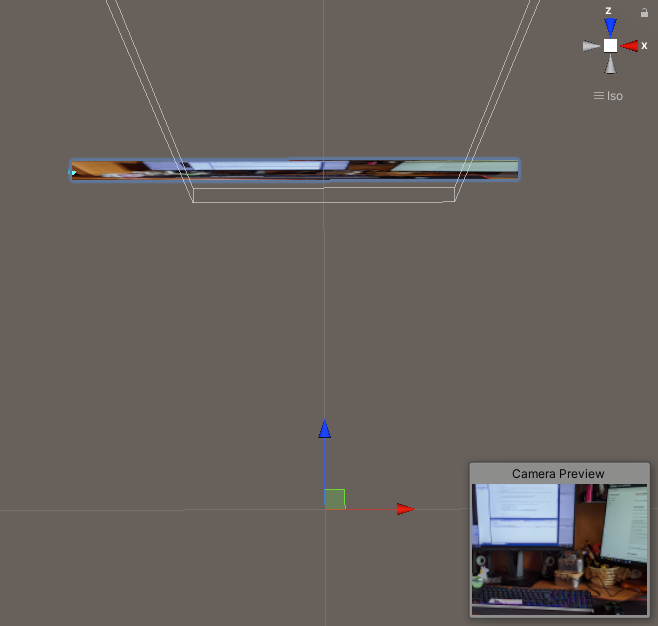
\includegraphics[width=0.7\textwidth]{images/canvasinyourfaceTopDown.PNG}
	\caption[Tiefe des Foto-Anzeige-Elements finden]{Die blaue Sphäre befindet sich nicht mehr in dem View Frustum und das Foto-Anzeige-Element befindet sich ein wenig hinter der Near Clipping Plane.}
	\label{illustration:canvasinsourfacetodown}
\end{figure}

Die Ränder des UI Elementes wurden genutzt, um die Intervalle für x und y zu bestimmen.
\begin{itemize}
	\item für x: [-0.2949, 0.2295]
	\item für y: [0.1546, -0.1507]
	\item Zusätzlich wurde z = -0.4 gesetzt. Das UI Element musste ein wenig weiter von der Clipping Plane entfernt sein um angezeigt zu werden.
\end{itemize}

Mit diesen Intervallen konnten DetectedObjects gut lokalisiert werden und es wurden keine Objekte mehr weggelassen, von denen der Nutzer erwarten würden, dass sie markiert werden.

\newpage
\section{Auswertung}

In diesem Kapitel geht es um die Evaluierung und Auswertung der vorgestellten Anwendung.

\subsection{Laufzeitanalyse}

Die Laufzeit der Objekterkennung wurde aufgezeichnet. Die Erkennung beginnt damit ein Foto aufzunehmen und endet mit der Erzeugung der Labels.

Die genutzte Netzwerkverbindung hatte eine Dowloadgeschwindigkeit von 180 Mbps und ein Uploadgeschwindigkeit von 18 Mbps.

Bilder haben Auflösung von 1090 x 1820 Pixel. Wenn sie in den HTTP-Anfragen verschickt haben, sie die Größe von 5 Mb.

Der Netzwerk Delay zwischen den REST-APIs und der Applikation wurde getestet, indem HTTP-Anfragen mit einem inkorrekten Authentifizierungsschlüssel gestellt wurden. In dem Body des Anfrage wurde ein Bild mitgeschickt, dieses wurde jedoch nicht analysiert. 

Im Durchschnitt beträgt die Round Trip Time 0,18 Sekunden in 14 Durchführungen dieses Tests. (Minimal 0,13 Sekunden, Maximal 0,28 Sekunden.)

Siehe Abbildung \ref{img:laufzeit}

\begin{figure}[H]
	\centering
	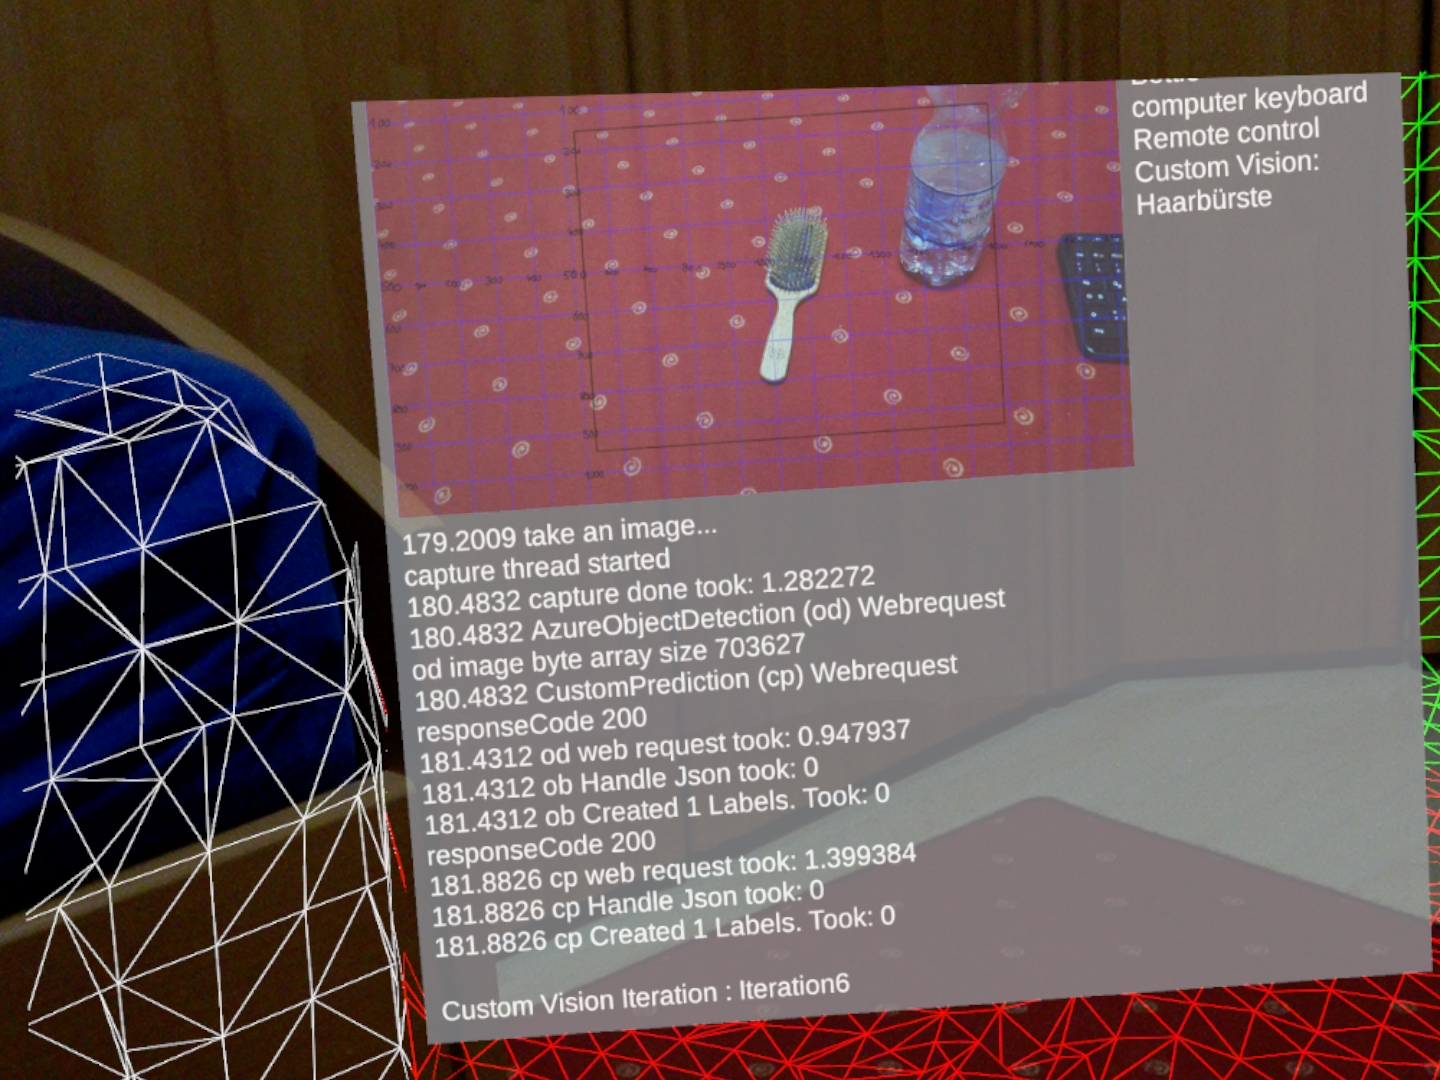
\includegraphics[width=0.9\textwidth]{images/ML_20201014_02.30.11.jpg}
	\caption[Laufzeit einer Objekterkennung]{Durchlauf mit Laufzeit Aufzeichnung}
	\label{img:laufzeit}
\end{figure}

Über 13 aufgenommene Fotos wurde festgestellt, dass das Aufnehmen des Fotos im Durchschnitt 1,11 Sekunden dauert. Die Anfragen an den Azure Object Detection Services, inklusive Netzwerk Response Time liegen Durchschnittlich bei 0,96 Sekunden. Die Anfragen an den Azure Custom Vision Service, inklusive Netzwerk Response Time, dauern im Durchschnitt 1,84 Sekunden. Für Azure Custom Vision wurde Iteration 6 verwendet. 

Azure Object Detection und Azure Custom Vision werden parallel zueinander in unterschiedlichen Threads durchgeführt. Die durchschnittliche Gesamtlaufzeit der Objekterkennung liegt bei 2,95 Sekunden.

Das Auslesen der Json Antworten, das Lokalisieren der Objekten in der 3D Szene und die Labelerstellung, benötigt weniger als eine Mikrosekunde. Siehe Abbildung \ref{table:laufzeitanalyse} und \ref{table:laufzeitanalyse2}.

\begin{figure}[H]
	\centering
	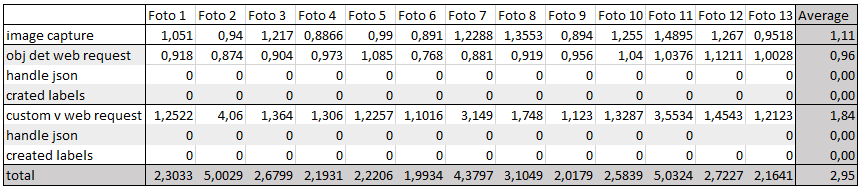
\includegraphics[width=1\textwidth]{images/table_Laufzeitanalyseneu.PNG}
	\caption[Laufzeitanalyse über 13 Bild-Analysen]{Laufzeitanalyse über 13 Bild-Analysen.}
	\label{table:laufzeitanalyse}
\end{figure}

\begin{figure}[H]
	\centering
	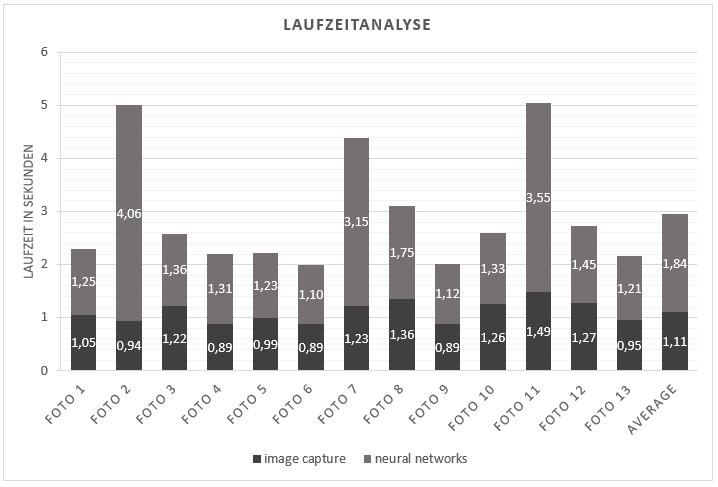
\includegraphics[width=0.95\textwidth]{images/table_Laufzeitanalyse2neu.PNG}
	\caption[Diagramm Laufzeitanalyse]{Diagramm Laufzeitanalyse}
	\label{table:laufzeitanalyse2}
\end{figure}

Der Prozess ist somit deutlich zu langsam um in Echtzeit ausgeführt zu werden. 

Ein einziges neuronales Netzwerk für die Objekterkennung zu verwenden, würde die Laufzeit verringern. Allerdings geht dann die Möglichkeit verloren, mehrere neuronale Netze zu verwenden die unterschiedliche Computer Vision Aufgaben erledigen. Aus einem RGB-Bild können beispielsweise mehr semantische Informationen extrahiert werden, wenn Image Segmentation und Object Detection kombiniert werden.

%Allerdings muss dann ein neuronales Netzwerk eingesetzt werden, dass speziell für die Applikation trainiert ist. Durch das verwenden von mehreren neuronalen Netzwerken besteht jedoch die Möglichkeit mehr semantische Informationen auf den RGB-Bilder zu erhalten als mit einem Netzwerk möglich wäre. So kann ein Netzwerk beispielsweise 

Neben den Objekterkennung-Prozessen braucht das Aufnehmen der Fotos mit durchschnittlich 0.9 Sekunden einen großen Teil der Laufzeit. Durch ein Umstieg von Fotos auf Frames eines Videostreams kann die Aufnahmezeit reduziert werden.  

%Durchschnittlich wurden durch Objekt Detection 1.64 Objekte pro Bild erkannt und durch Custom Detection 0.73.

\subsection{Evaluierung der Objekterkennung durch Azure Objekt Detection}

Die Anwendung wurde in einem Schlaf- und Arbeitszimmer getestet. Durch Azure Object Detection konnten folgende Object-Klasse erkannt werden: Television, Person, Bottle, Keyboard, Computermouse, cat, bed, luggage, chair, laptop.

Azure Object Detection erkennt die Objekte mit unterschiedlicher Verlässlichkeit. Tastaturen und Personen wurden in den meisten Aufnahmen korrekt erkannt. Das Lightwear Gerät der Magic Leap One wurde gelegentlich als Computermaus interpretiert und Computerbildschirme wurden durchweg als Television oder als Laptop markiert.

\subsection{Evaluierung der Objekterkennung durch Azure Custom Vision}

Die Genauigkeit der Objekterkennungen durch Azure Custom Vision wird durch das Training des Modells bestimmt. Dieser Cloud Service hat sich als effektiv erweisen, um Azure Object Detection zu ergänzen. Mit der Iteration 6, die mit 51 Bildern eine Stunde lang trainiert wurde, kann die Haarbürste zuverlässig erkannt werden. 

Für Regionen in denen sich keine Haarbürste befindet, berechnet das Modell eine Probability von weniger als 5 Prozent dafür, dass sich dort fälschlicherweise eine Haarbürste befindet. 

Regionen, die mit einer Probability von über 50 Prozent einer Haarbürste enthalten, beinhalteten in der Anwendung immer eine Haarbürste.

Durch die niedrige Rate an false positives konnte die Akzeptanzschwelle auf 60 Prozent gesetzt werden, um die Rate der false negatives zu verringern. Dadurch wird die Haarbüste fast immer korrekt erkannt, wenn sie auf einem Bild ist.


\subsection{Objekte in 3D Szene lokalisieren}

In diesem Teil wird evaluiert wie akkurat Objekte, die in einem Foto erkannt wurden, in der 3D Umgebung markiert werden.
Um die Lokalisierung zu evaluieren, wurden die RGB-Bild festgehalten, mit denen Objekterkennung durchgeführt wurde. Auf den RGB-Bildern wurde der Mittelpunkt der Bounding Boxen markiert. Siehe Abbildung \ref{img:markedonimage}. Das Label, das in der Szene gesetzt wird, soll mit dieser Position korrespondieren. Siehe Abbildung \ref{img:labelsszene}. 
\begin{figure}[H]
	\centering
	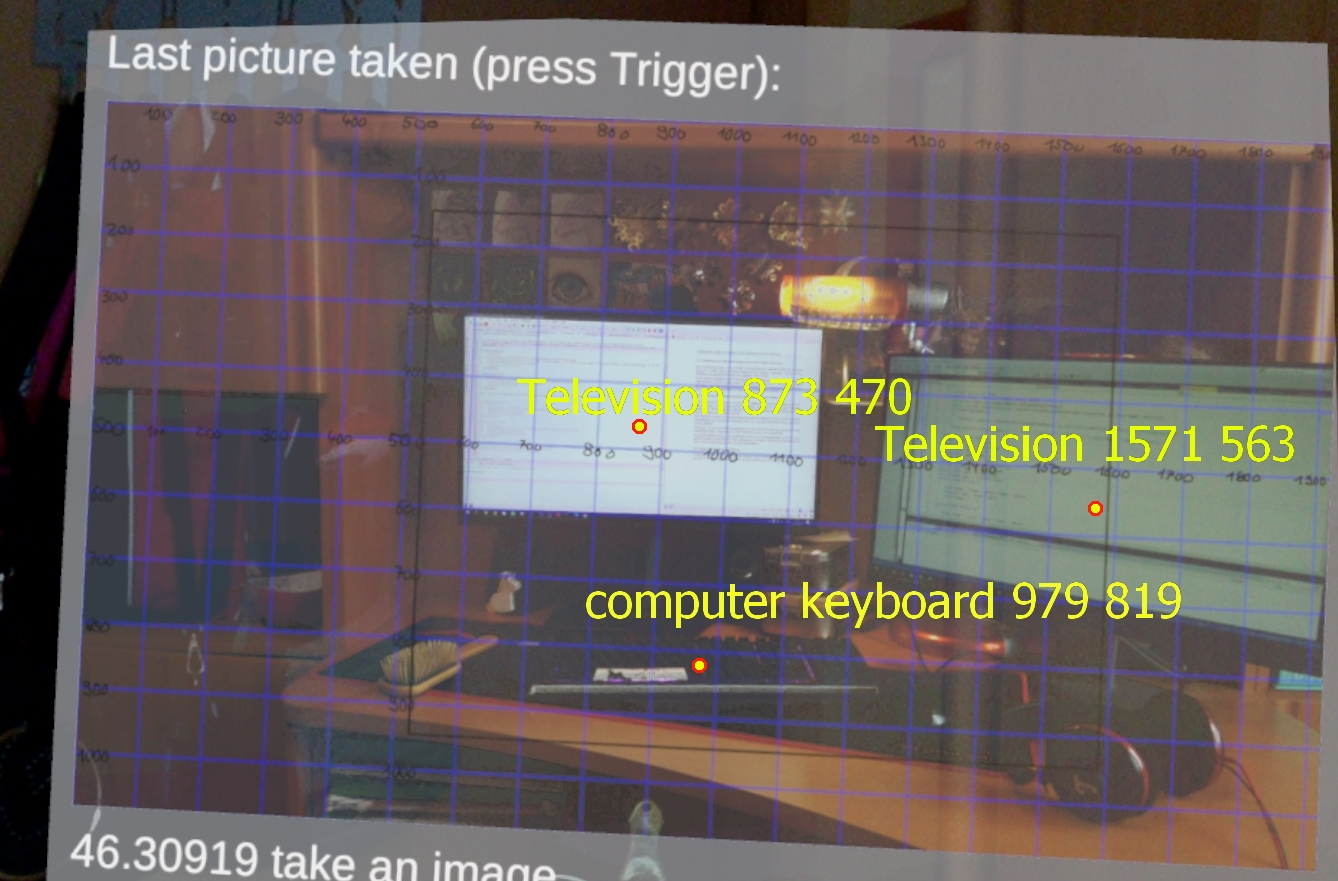
\includegraphics[width=0.8\textwidth]{images/ML_markedOnImage2.jpg}
	\caption[Erkennt Objekte auf RGB-Bilde markiert]{Die Mittelpunkte der erkannten Objekte wurden, auf dem Foto per Hand in rot-gelb markiert. Die Klassen und die u,v Foto-Koordinaten der Objekten sind angegeben.}
	\label{img:markedonimage}
\end{figure}

\begin{figure}[H]
	\centering
	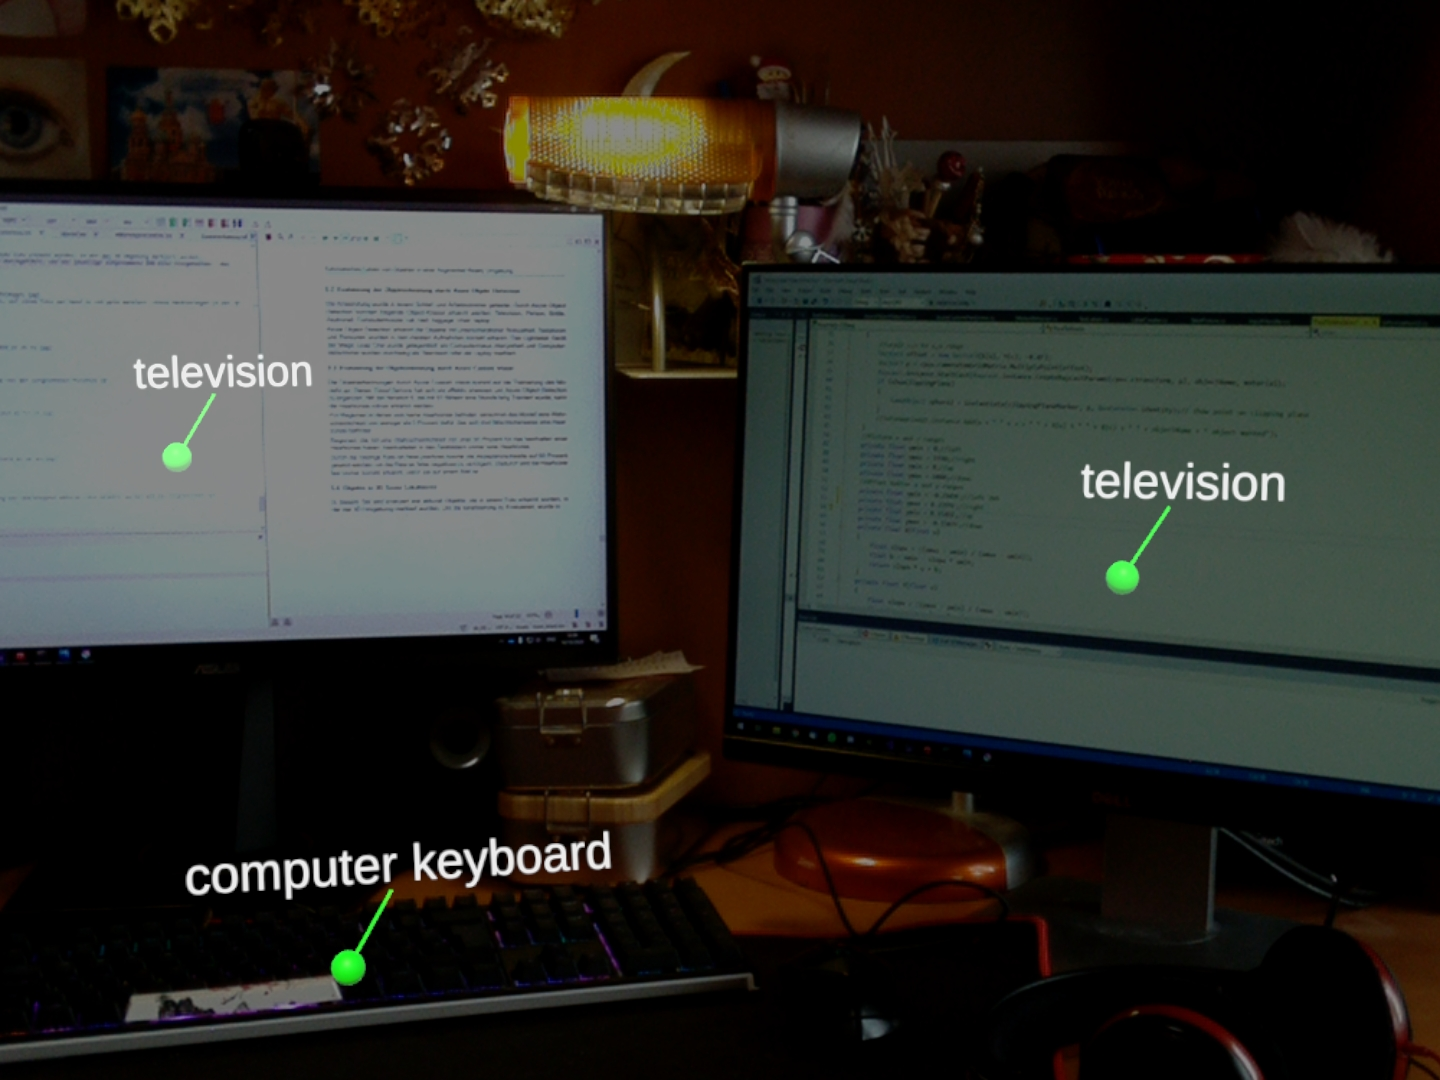
\includegraphics[width=0.8\textwidth]{images/ML_20201014_13.39.00.jpg}
	\caption[Erkannte Objekte in der Szene markiert]{Objekte in der 3D Szene markiert.}
	\label{img:labelsszene}
\end{figure}

Die Positionierungen der Labels weichen um weniger als 2 cm von der vorgesehenen Position ab.


%\begin{figure}[H]
%	\centering
%	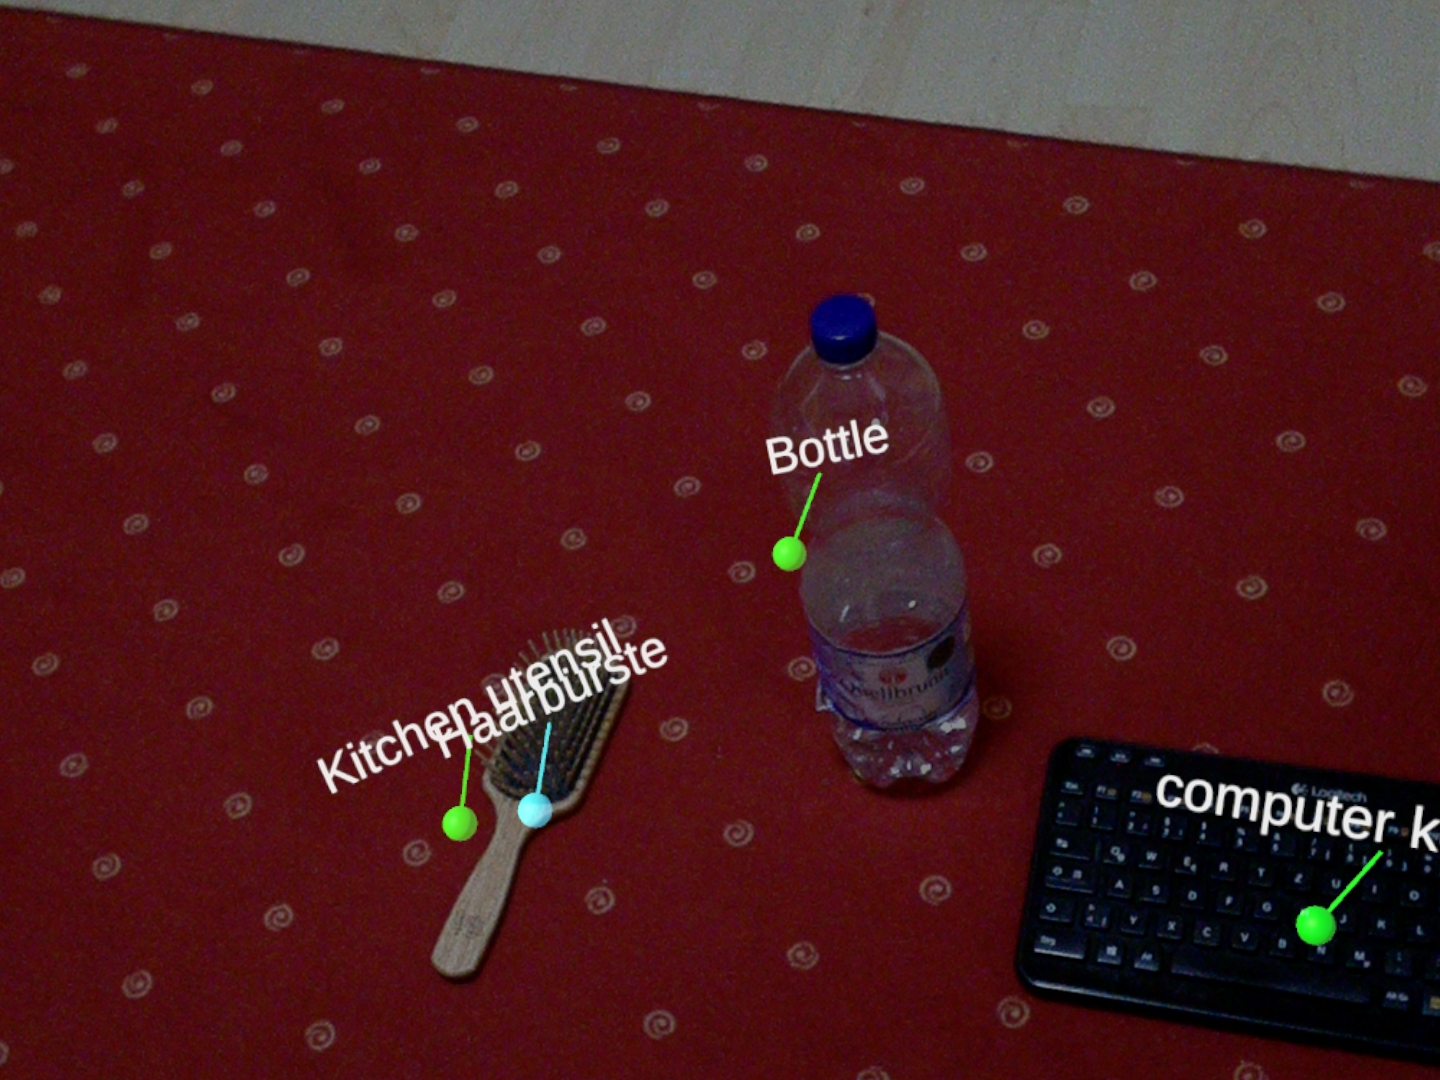
\includegraphics[width=0.95\textwidth]{images/ML_20201014_02.57.37.jpg}
%	\caption[]{erste erkennung}
%	\label{table:laufzeitanalyse2}
%\end{figure}
%
%\begin{figure}[H]
%	\centering
%	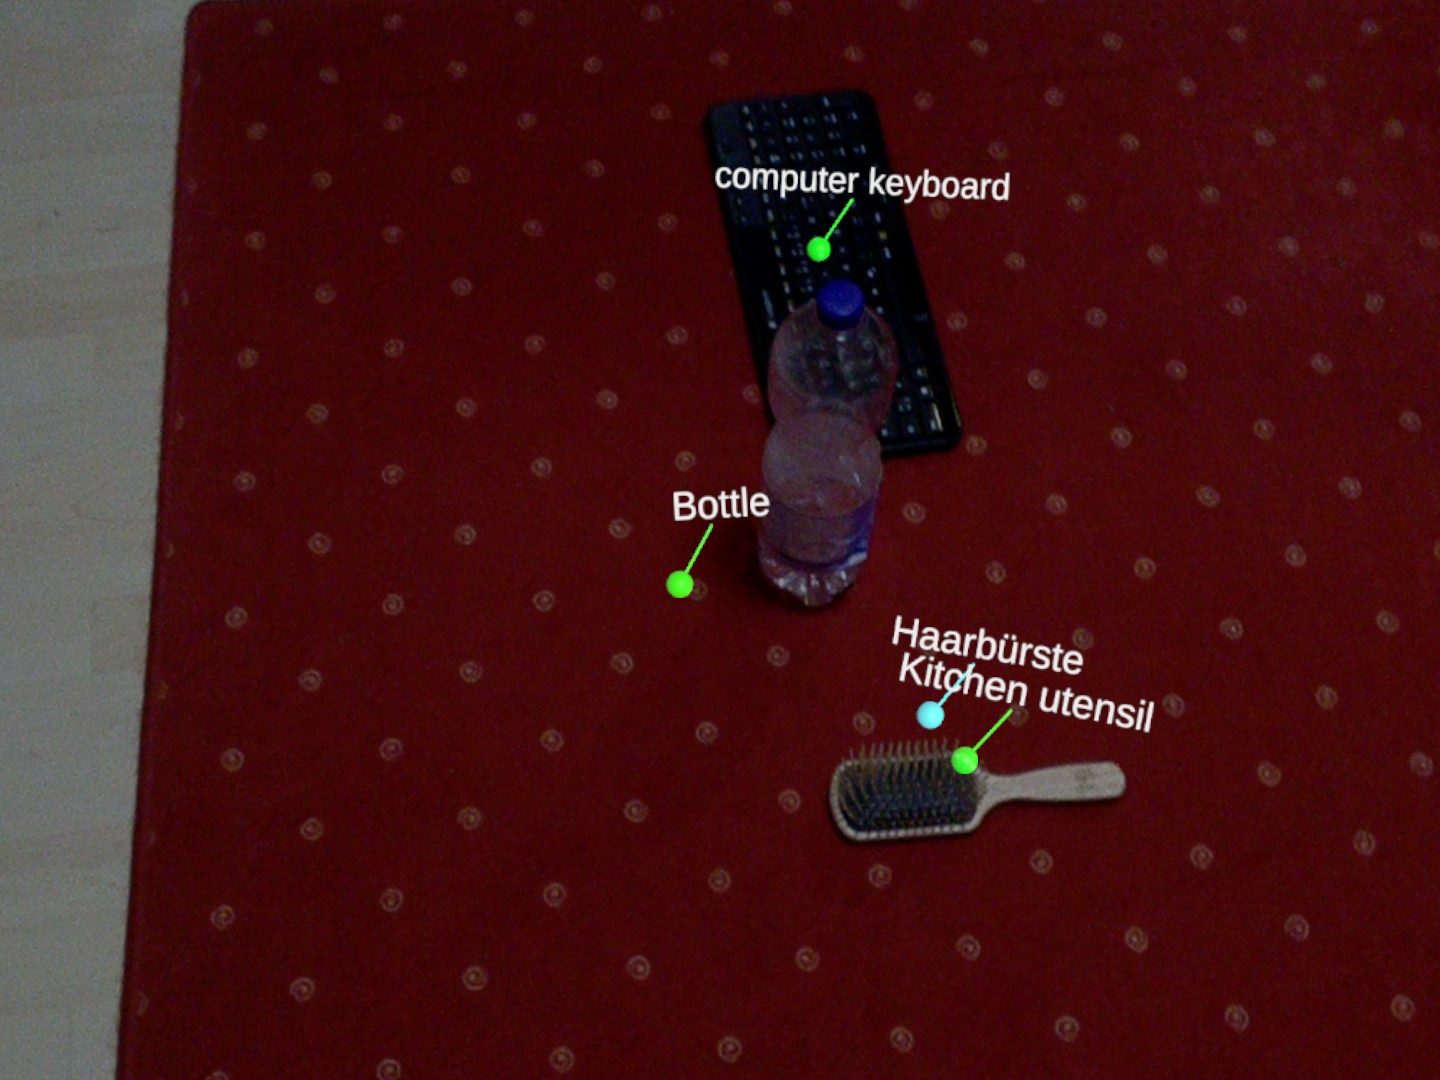
\includegraphics[width=0.95\textwidth]{images/ML_20201014_02.58.02.jpg}
%	\caption[]{zweite erkennung}
%	\label{table:laufzeitanalyse2}
%\end{figure}

Die Lokalisierung der Objekte hängt von dem geometrischen Verständnis der AR-Brille an. Objekte die häufig bewegt werden, wie beispielsweise ein Stuhl, werden erst in die Spatial Map eingefügt, wenn sie über längere Zeit nicht bewegt wurden. Das Einfügen des Objektes in die Map dauert ca. 2 Minuten. 

Wenn der Objekte Detection Prozess auf ein Objekt angewandt wird, das noch nicht oder nicht komplett in der Spatial Map ist, wird es nicht korrekt markiert. Siehe Abbildung \ref{img:stuhl}. 

\begin{figure}[H]
	\centering
	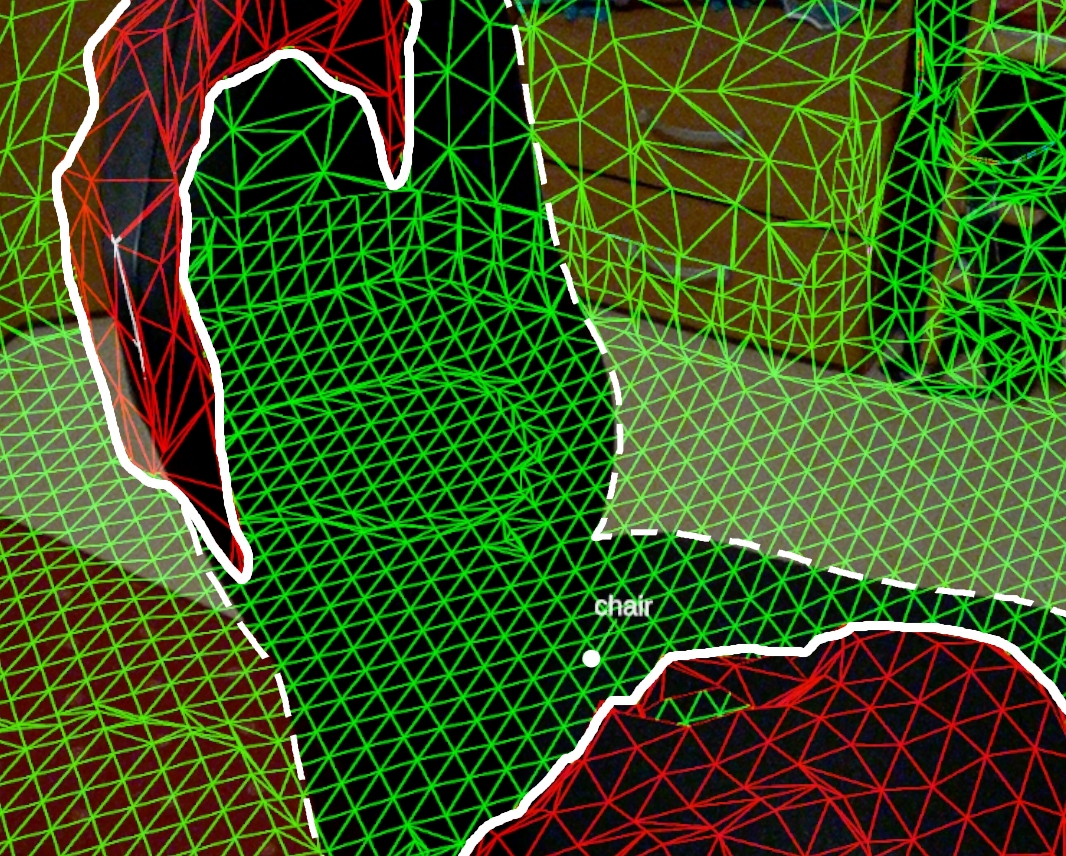
\includegraphics[width=0.8\textwidth]{images/ML_20201004_19.18.02_sup.jpg}
	\caption[Label  setzten, bei fehlerhafter Spatial Map]{Spatial Map des Stuhles in weiß umrandet. Tatsächlicher Stuhl in orange umrandet. Label des Stuhls in gelb markiert. Das Label befindet sich in der Szene hinter dem Stuhl auf dem Boden.}
	\label{img:stuhl}
\end{figure}

In diesem Beispiel ist ein Stuhl noch nicht in der Spatial Map. Wenn die Applikation einen Raycast auf die Umgebung durchführt, um das gefundene Objekt zu markieren, schießt der Raycast durch das tatsächliche Objekte hindurch, da es  nicht in der Map ist. Der Raycast trifft den Boden hinter dem Objekt und markiert diesen. Der Stuhl wurde von der Objekterkennung korrekt erkannt, jedoch nicht korrekt in der Szene markiert.

Halb transparente Objekte werden ebenfalls nicht korrekt gemapped. Daher wird das Label eines Flaschen-Objekts nicht korrekt positioniert. Siehe Abbildung \ref{img:flasche}.

\begin{figure}[H]
	\centering
	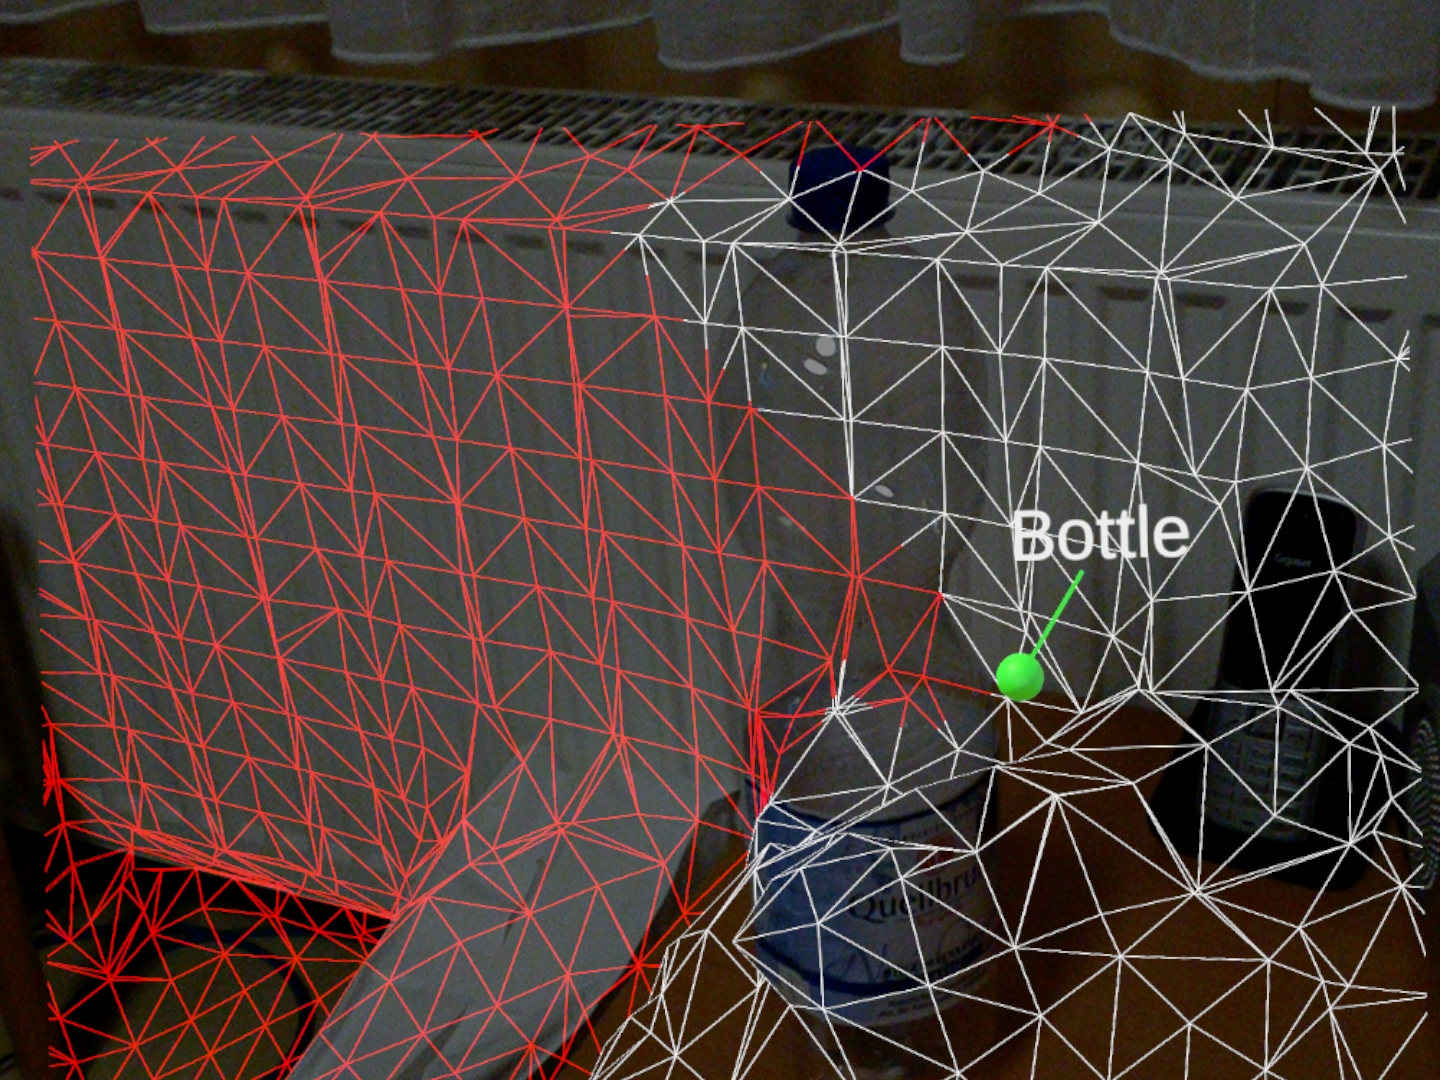
\includegraphics[width=0.8\textwidth]{images/ML_20201004_19.12.13.jpg}
	\caption[Spatial Mapping Transparenter Objekte]{Das Label für Bottle liegt hinter dem tatsächlichen Objekt. Die Flasche wurde nicht korrekt gemapped.}
	\label{img:flasche}
\end{figure}
